\documentclass[a4paper, 10pt]{article}

% ==========================================
% 1. PAGE GEOMETRY & LAYOUT
% ==========================================
\usepackage[left=1.5cm, right=1.5cm, top=2cm, bottom=2cm]{geometry} 
\usepackage{multicol} 
\setlength{\columnsep}{1cm} 

% ==========================================
% 2. TYPOGRAPHY & MATH FONTS
% ==========================================
\usepackage[T1]{fontenc}
\usepackage{lmodern}
\usepackage{amsmath} % Load amsmath BEFORE mathdesign
\usepackage[bitstream-charter]{mathdesign}
\usepackage{microtype} % Improves text justification and spacing

% ==========================================
% 3. GRAPHICS & FLOATS (Images & Tables)
% ==========================================
\usepackage{graphicx}
\usepackage{caption}
\usepackage{float} % Required for forcing image/algorithm placement with [H]

% ==========================================
% 4. ALGORITHMS
% ==========================================
\usepackage{algorithm}
\usepackage{algpseudocode}

% ==========================================
% 5. SOURCE CODE LISTINGS (Dynamic Tomorrow Night Blue - No Background)
% ==========================================
\usepackage{xcolor}
\usepackage{listings}

% Adapted Tomorrow Night Blue palette for a white/transparent background
\definecolor{tnbText}{HTML}{002451}      % Signature Deep Blue (Main Text)
\definecolor{tnbComment}{HTML}{7285b7}   % Soft Blue-Grey (Comments)
\definecolor{tnbKeyword}{HTML}{8959a8}   % Dynamic Purple (Keywords)
\definecolor{tnbString}{HTML}{3e999f}    % Teal/Aqua (Strings)
\definecolor{tnbNumber}{HTML}{f5871f}    % Orange (Numbers)

% Define the crisp JS Style
\lstdefinestyle{jsStyle}{
    language=Java, % Uses Java base for JS syntax highlighting
    basicstyle=\ttfamily\small\color{tnbText},
    backgroundcolor=, % BLANK = NO BACKGROUND COLOR
    commentstyle=\color{tnbComment}\itshape,
    keywordstyle=\color{tnbKeyword}\bfseries,
    stringstyle=\color{tnbString},
    numberstyle=\tiny\color{tnbNumber},
    identifierstyle=\color{tnbText},
    breakatwhitespace=false,         
    breaklines=true,                 
    frame=single,
    rulecolor=\color{tnbComment}, % Makes the border line a soft blue-grey
    captionpos=b,                    
    keepspaces=true,                 
    showspaces=false,                
    showstringspaces=false,
    showtabs=false,                  
    tabsize=2
}
% Apply the style globally
\lstset{style=jsStyle}

% ==========================================
% 6. BIBLIOGRAPHY (IEEE Style)
% ==========================================
\usepackage[style=ieee, sorting=none]{biblatex} 
\addbibresource{references.bib} 

% ==========================================
% 7. HYPERLINKS (MUST ALWAYS BE LAST!)
% ==========================================
\usepackage{hyperref}
\hypersetup{
    colorlinks=true,   % Removes ugly default boxes
    linkcolor=cyan,    % Color for internal links (Figures, Sections)
    citecolor=cyan,    % Color for citations [1]
    urlcolor=cyan      % Color for web URLs
}

\begin{document}
% ==========================================
% 1-COLUMN SECTION (Full Width)
% ==========================================
\title{\textbf{Vectra:} The Quarantine Matrix, Constraining Neural Hallucinations in \\ 3D Gaussian Environments}

% All caps for the name, italicized for the university
\author{PARSA BESHARAT, \textit{Technische Universität Bergakademie Freiberg, Germany} \\
\textit{\href{mailto:parsabe99@gmail.com}{\url{parsabe99@gmail.com}}} \\
\textit{\url{https://vectra.parsabe.com/}}}


\date{} 

\maketitle

\begin{figure}[h!]
    \centering
   \includegraphics[width=\textwidth]{img/logo.png}
    
\caption{Created by Google Gemini - Vectra logo.}
\end{figure}

    
% Anything placed here, like your title and teaser image, spans the whole page.

\begin{multicols}{2}

\begin{center}
 \Large\textbf{Abstract}
\end{center}

\noindent The hyper-accelerated rise of generative artificial intelligence is rewiring the rules of 3D content creation. Yet, seamlessly jacking everyday 2D inputs---like text prompts and flat images---into fully interactive, dynamic 3D constructs remains a critical bottleneck. This paper introduces an end-to-end framework engineered to generate, extract, and simulate high-fidelity 3D objects directly from simple visual and textual data. By harnessing advanced neural rendering and spatial splatting algorithms, our system spins up robust 3D assets on the fly, entirely bypassing the tedious grind of traditional manual modeling. We orchestrate a streamlined pipeline that fuses zero-shot semantic extraction, generative mesh synthesis, and web-based physics integration. This unified architecture doesn't just supercharge the rendering of complex 3D scenes; it breathes real-time kinetic life into them, enabling fluid dynamic simulation and direct user manipulation. We benchmark the framework’s performance across structural integrity, pipeline latency, and interactive immersion within a scalable network. Ultimately, this work delivers a highly optimized, plug-and-play solution that accelerates the 3D creation workflow, paving the way for the next generation of accessible, dynamic, and fully interactive digital realities. This project is available on the website: \url{https://vectra.parsabe.com}


\section{INTRODUCTION}
The boundary between the physical world and the digital grid is dissolving. As we push further into immersive virtual spaces, the demand for high-fidelity, three-dimensional constructs is skyrocketing. We are no longer satisfied with flat screens and 2D interfaces; the future is built on spatial computing, where digital objects occupy virtual volume. However, populating this new frontier is a massive bottleneck. This paper introduces a streamlined, end-to-end framework designed to shatter that bottleneck, allowing users to jack simple 2D inputs---like text prompts or flat images---directly into fully interactive, dynamic 3D realities.

\subsection{Background and Motivation}
The recent explosion of generative artificial intelligence has fundamentally rewired how we create digital content. Neural networks can now dream up hyper-realistic images and text in milliseconds. Yet, the leap from 2D pixels to 3D polygons remains one of the hardest problems in computer vision.

Historically, crafting 3D assets required digital artisans to spend hours, if not days, manually sculpting meshes, baking textures, and rigging physics. As the demand for virtual environments, digital twins, and interactive simulations explodes, this manual grind is no longer sustainable. The motivation behind this work is to automate the forge. By leveraging neural rendering and advanced spatial algorithms, we aim to democratize 3D creation---allowing anyone with a text prompt or a single image to instantly manifest objects into the digital realm.

\subsection{Problem Statement}
The core problem is translation: how do you force a flat, 2D data source to project a fully realized 3D construct accurately?

While early neural rendering techniques and primitive generative models have made strides, they suffer from critical flaws. They are often computationally heavy, requiring massive processing power and long rendering times that kill real-time workflow. Worse, the outputs are usually ``dead'' assets---static, rigid point clouds or messy meshes that look fine from one angle but completely break down when you try to move them, edit them, or drop them into a physics engine. To build truly interactive worlds, we do not just need 3D shapes; we need functional, optimized assets that can collide, fall, and respond to virtual physics in real time.

\subsection{Key Contributions}
To solve these massive computational bottlenecks, this paper proposes a unified, highly optimized architecture. Our system seamlessly bridges the gap between raw generative AI and functional 3D simulation. Our key contributions include:

\begin{itemize}
    \item \textbf{Zero-Shot Semantic Extraction Pipeline:} A method to intelligently carve out and isolate target objects from messy, in-the-wild 2D images without requiring pre-trained, scene-specific data.
    \item \textbf{Rapid Image-to-3D and Text-to-3D Synthesis:} A cloud-proxy architecture that leverages isolated 2D generation models alongside advanced splatting algorithms to rapidly hallucinate 3D geometry from minimal input.
    \item \textbf{Generative Mesh Optimization:} A highly efficient protocol for synthesizing clean, lightweight 3D meshes that retain high-fidelity textures while being perfectly optimized for real-time rendering environments.
    \item \textbf{Kinetic Physics Integration:} A web-based dynamic framework that injects the newly forged 3D meshes with real-time physical properties, allowing them to instantly interact, collide, and exist within simulated virtual environments.
\end{itemize}

\section{RELATED WORKS}
In the foundational work \cite{mildenhall2020nerf}, Mildenhall et al., the authors in the paper titled \textit{NeRF: Representing Scenes as Neural Radiance Fields for View Synthesis}, proposed a radical new paradigm for constructing digital realities. Instead of relying on traditional 3D polygons or discrete point clouds, they tackled the problem of novel view synthesis by training an AI to hallucinate a continuous, volumetric hologram of a scene.

They accomplished this by modeling the physical environment as a continuous 5D mathematical function. The system feeds a deep, fully-connected neural engine (a Multilayer Perceptron, devoid of standard convolutional layers) a precise 5D coordinate: a specific spatial location in the 3D grid $(x, y, z)$, coupled with the user's exact viewing angle $(\theta, \phi)$. In return, the neural network calculates two crucial variables for every microscopic point in that space:

\begin{enumerate}
    \item \textbf{Volume Density:} A differential opacity value that dictates how ``solid'' or transparent the space is.
    \item \textbf{Radiance:} The view-dependent RGB color that the point emits.
\end{enumerate}

To project this Neural Radiance Field into a visible 2D image from any new angle, the framework executes a strict three-step protocol:

\begin{enumerate}
    \item \textbf{Ray Marching:} The system fires virtual camera rays deep into the digital void, sampling a set of 3D coordinates along each ray's trajectory.
    \item \textbf{Neural Querying:} It jacks those sampled points and their corresponding viewing angles directly into the neural network to extract the predicted colors and opacities.
    \item \textbf{Volume Accumulation:} Using classical volume rendering techniques, the system compresses those floating data points along the ray, fusing them into a final, crisp 2D pixel grid.
\end{enumerate}

Because this entire pipeline is fully differentiable, the machine can self-correct. The algorithm relentlessly calculates the error between its synthetic renders and the actual captured source photographs. By using gradient descent to minimize this error across dozens of viewpoints, the network organically learns to lock high densities and photorealistic colors exactly where the true physical objects exist, weaving a hyper-accurate 3D construct from sparse 2D data.

They encode the continuous physical grid as a 5D vector-valued function. The input stream requires a 3D spatial coordinate $x$ and a 2D viewing vector $(\theta, \phi)$, terminating in an output construct of emitted color $c = (r,g,b)$ and structural volume density $\sigma$. In the field, they strip the viewing angle down, expressing the direction as a 3D Cartesian unit vector $d$. 

They hardwire this continuous 5D holographic representation into an MLP neural engine defined as $F_\Theta : (x,d) \rightarrow (c,\sigma)$. By relentlessly optimizing its synaptic weights $\Theta$, the daemon maps each raw 5D input coordinate to its exact localized density and directional color emission. They force the representation to maintain strict multiview consistency by choking the network's prediction logic: the structural volume density $\sigma$ is locked as a function of only the spatial location $x$. Meanwhile, the RGB color signature $c$ is unshackled, allowed to shift dynamically based on both the location in the void and the observer's viewing direction. 

To execute this protocol, the MLP daemon $F_\Theta$ first ingests the input 3D coordinate $x$ and feeds it through a deep gauntlet of 8 fully-connected layers (running ReLU activations across a massive 256-channel bandwidth per layer). This calculates the density $\sigma$ alongside a dense 256-dimensional feature vector. Finally, this feature payload is spliced together with the camera ray's viewing trajectory and jacked into one final, specialized fully-connected layer (using a ReLU activation and a tighter 128-channel bottleneck) to synthesize the final, view-dependent RGB color output.

\begin{figure*}[t] 
    \centering
    
\includegraphics[width=\textwidth]{img/1.png} 
    
    \caption{An overview of their neural radiance field scene representation and differentiable rendering procedure. They synthesize images by sampling 5D coordinates (location and viewing direction) along camera rays (a), feeding those locations into an MLP to produce a color and volume density (b), and using volume rendering techniques to composite these values into an image (c). This rendering function is differentiable, so they can optimize their scene representation by minimizing the residual between synthesized and ground truth observed images (d). \cite{mildenhall2020nerf}.}
    \label{fig:nerf_overview}
\end{figure*}

The 5D neural radiance matrix represents a physical construct as a continuous field of volume density and directional emitted radiance across any point in the digital void. They synthesize the chromatic signature of any tracer ray piercing the scene using legacy protocols from classical volume rendering [16]. The structural density $\sigma(x)$ acts as the differential probability of a ray slamming into a microscopic data-particle exactly at spatial coordinate $x$. The predicted optical payload $C(r)$ of a virtual camera ray $r(t) = o+td$, constrained by the near and far clipping bounds $t_n$ and $t_f$, is defined as:

\begin{equation}
\begin{split}
C(\mathbf{r}) &= \int_{t_n}^{t_f} T(t) \sigma(\mathbf{r}(t)) \mathbf{c}(\mathbf{r}(t), \mathbf{d}) dt \;, \\
&\text{where } T(t) = \exp\left( - \int_{t_n}^{t} \sigma(\mathbf{r}(s)) ds \right) .
\end{split}
\end{equation}

The decay function $T(t)$ defines the accumulated transmittance along the trajectory from $t_n$ to $t$---essentially the statistical odds that the signal survives the jump from $t_n$ to $t$ without colliding with rogue geometry. Rendering a visual feed from their continuous neural hologram requires estimating this integral $C(r)$ for every single optic ray fired through the pixel grid of the virtual viewport.

They brute-force this continuous integral using numerical quadrature. Legacy deterministic quadrature, typically used to render primitive discretized voxel grids, would severely throttle their construct's resolution, as the MLP daemon would only be pinged at a rigid, hardcoded array of locations. To bypass this bottleneck, they execute a stratified sampling protocol: they slice the vector interval $[t_n,t_f]$ into $N$ evenly-spaced memory bins, and then pull one sample uniformly at random from deep within each bin:

\begin{equation}
t_i \sim \mathcal{U} \left[ t_n + \frac{i-1}{N}(t_f - t_n), \; t_n + \frac{i}{N}(t_f - t_n) \right] .
\end{equation}

\subsection{Evaluation Metrics}
Synthesizing novel visual feeds via NeRF protocols requires strict quality assessment telemetry to benchmark the matrix. These diagnostics evaluate the fidelity of individual holo-frames using either full-reference crosschecks (against ground-truth source data) or zero-reference blind estimations. As documented in their extensive network audit \cite{rabby2024beyondpixels}, the most widely deployed metrics for evaluating these neural constructs are Peak Signal to Noise Ratio (PSNR), Structural Similarity Index Measure (SSIM), and Learned Perceptual Image Patch Similarity (LPIPS).

\subsubsection{Peak Signal to Noise Ratio (PSNR)}
Peak Signal to Noise Ratio (PSNR) operates as a full-reference quality diagnostic, calculating the digital distortion between the pristine reference file and the hallucinated image. The computation is driven by the ratio of the highest attainable signal threshold to the mean squared error (MSE) between the two datastreams:

\begin{equation}
PSNR(I) = 10 \cdot \log_{10} \left( \frac{MAX(I)^2}{MSE(I)} \right)
\end{equation}

Here, $MAX(I)$ represents the absolute maximum possible pixel value within the visual matrix, and $MSE(I)$ denotes the pixel-wise mean squared error audited across all color channels. PSNR remains a heavily utilized standard across NeRF research and broader signal-processing fields. While a higher PSNR readout guarantees a lower baseline error and a structurally superior render, the metric has limits. It relies on raw mathematical variance and is notoriously blind to subtle perceptual shifts in the grid, such as micro-fluctuations in brightness, contrast, or saturation.

\subsubsection{Structural Similarity Index Measure (SSIM)}
The Structural Similarity Index Measure (SSIM) operates as a full-reference diagnostic designed to measure the structural integrity between the pristine reference matrix and the synthesized visual feed. SSIM is defined as the product of two core vectors: local similarity and contrast similarity. Local similarity audits the localized pixel intensities between the two constructs, while contrast similarity evaluates their localized contrast differentials. A higher SSIM readout signals a superior structural lock between the two images, resulting in a cleaner holo-render. Unlike the brute-force PSNR, SSIM is hyper-sensitive to subtle structural mutations in the digital grid, though this precision comes at the cost of heavier computational overhead.

\begin{equation}
SSIM(x, y) = \frac{(2\mu_x\mu_y + C_1)(2\sigma_{xy} + C_2)}{(\mu_x^2 + \mu_y^2 + C_1)(\sigma_x^2 + \sigma_y^2 + C_2)}
\end{equation}

The SSIM diagnostic quantifies the similarity between two images $x$ and $y$ by cross-referencing their statistical properties. This includes their localized means ($\mu_x$ and $\mu_y$), internal variances ($\sigma_x^2$ and $\sigma_y^2$), and the structural covariance ($\sigma_{xy}$) bridging them. Additionally, $C_1$ and $C_2$ act as stabilizing constants, preventing catastrophic division by near-zero variances and ensuring absolute numerical stability during the computation cycle. Ultimately, this equation provides a strict, quantitative audit of how closely two visual constructs match in terms of fundamental structure and texture.

\subsubsection{Learned Perceptual Image Patch Similarity (LPIPS)}
The Learned Perceptual Image Patch Similarity (LPIPS) is a highly advanced, full-reference quality diagnostic that deploys a deep neural network daemon to calculate perceptual similarity between visual feeds. It is engineered to detect microscopic anomalies and subtle perceptual shifts that slip past legacy metrics like PSNR and SSIM. LPIPS stands as the bleeding-edge standard for perceptual sensitivity, though it burns through massive amounts of computational power to execute. The LPIPS score is derived from the weighted pixel-wise Mean Squared Error (MSE) of feature maps ripped across multiple network layers. Unlike earlier metrics, a lower LPIPS value flags a tighter perceptual lock between the constructs and a higher-fidelity render.

\begin{equation}
LPIPS(x, y) = \sum_{l=1}^L \frac{1}{H_l W_l} \sum_{h=1}^{H_l} \sum_{w=1}^{W_l} ||w_l (x_{lhw} - y_{lhw})||_2^2
\end{equation}

Here, $x_{lhw}$ and $y_{lhw}$ represent the deep features extracted from the pristine reference and the assessed image, locked at the spatial coordinates $(w, h)$ within layer $l$. The variables $H_l$ and $W_l$ dictate the precise spatial dimensions (height and width) of the feature map operating at that specific layer $l$.

\subsection{Vulnerabilities in Few-Shot Synthesis: The Need for Constrained Algorithms}
Synthesizing novel visual vectors becomes a severe computational bottleneck when the target physical space is only sparsely observed. Baseline systems like NeRF, which train isolated networks on individual scenes, struggle to function without prior structural knowledge inherited from similar environments. As documented by Jain et al. \cite{jain2021dietnerf}, the foundational NeRF matrix suffers catastrophic failures during few-shot novel view synthesis across multiple settings, serving as the primary motivation for constrained, semantically-aware algorithms like DietNeRF.

\textbf{Overfitting to Sparse Data Streams:} 
A critical vulnerability emerges when the network overfits to its limited training feeds. Conceptually, the daemon learns by mimicking the image-formation process at strictly observed poses. The radiance field is calculated by repeatedly sampling a training image and its specific pose $(I, \mathbf{p}_i)$, rendering a synthetic image $\hat{I}_{\mathbf{p}_i}$ from that exact same spatial anchor via volume integration, and then minimizing the mean-squared error (MSE) between the two matrices to force pixel-wise alignment:

\begin{equation}
\mathcal{L}_{\text{full}}(I, \hat{I}_{\mathbf{p}_i}) = \frac{1}{HW} \| I - \hat{I}_{\mathbf{p}_i} \|_2^2
\end{equation}

In the field, to bypass the massive processing burn required to render full holo-frames during the training cycle, the framework subsamples a tighter batch of tracer rays $\mathcal{R}$ cast from the virtual cameras. Given these subsampled rays, the daemon minimizes the following loss function:

\begin{equation}
\mathcal{L}_{\text{MSE}}(\mathcal{R}) = \frac{1}{|\mathcal{R}|} \sum_{\mathbf{r} \in \mathcal{R}} \| \mathbf{C}(\mathbf{r}) - \hat{\mathbf{C}}(\mathbf{r}) \|_2^2
\end{equation}

When fed a dense array of training views, $\mathcal{L}_{\text{MSE}}$ provides a robust training signal deep into the volume without overfitting. The MLP successfully maps accurate textures and spatial occupancy, effectively utilizing sinusoidal positional embeddings to learn high-frequency functions and lock in fine details. Unfortunately, Jain et al. \cite{jain2021dietnerf} highlight that this exact high-frequency representational capacity becomes a fatal liability when only a few views are available. The $\mathcal{L}_{\text{MSE}}$ can be artificially minimized by packing the geometric reconstruction right up against the camera lens. The representation suffers from a near-field ambiguity, yielding degenerate solutions characterized by corrupted, skewed geometry and highly opaque artifacts that blind the virtual cameras.

\textbf{The Regularization Trade-off:} 
Attempts to patch this vulnerability via standard structural regularization—such as stripping out hierarchical sampling, relying on a single MLP, or throttling the maximum frequency positional embeddings—only create new compromises. While these patches successfully force the matrix to recover plausible base geometry by biasing the network toward lower-frequency solutions, the high-frequency, razor-sharp details are permanently wiped from the digital grid.

\textbf{Zero Prior Knowledge and Generalization Failure:} 
Furthermore, because the baseline NeRF daemon is initialized from absolute scratch for every new construct, it possesses zero prior knowledge regarding natural object symmetries or standard physics. When the network is trained exclusively on one side of a target asset, it completely fails to hallucinate the unseen geometry on the opposite side, as the $\mathcal{L}_{\text{MSE}}$ receives zero supervisory signals from the unobserved void. This necessitates the deployment of more advanced, semantically consistent architectures capable of hallucinating missing data structures from minimal input.

\subsection{Semantically Consistent Radiance Fields: The DietNeRF Protocol}
To combat the catastrophic geometry collapse in sparse data environments, more resilient, semantically-aware architectures were forged in the grid. While multiple experimental protocols have attempted to patch these few-shot vulnerabilities, one of the most robust breakthroughs is the DietNeRF construct introduced by Jain et al. \cite{jain2021dietnerf}. 

Motivated by the inherent limitations of isolated scene training, DietNeRF jacks in prior knowledge extracted from a pre-trained, heavy-duty image encoder. This external cognitive architecture acts as a stabilizing guide for the NeRF optimization sequence when operating in restrictive, few-shot parameters.

\subsubsection{Semantic Consistency Loss}
The DietNeRF daemon supervises the neural engine $f_\theta$ at arbitrary, unobserved camera poses by injecting a semantic consistency loss constraint. While brute-force pixel-wise comparisons (via standard $\mathcal{L}_{\text{MSE}}$) between ground-truth source data and synthetic renders only function when the generated image perfectly aligns with a pre-observed pose, the human optical cortex easily detects whether two images represent the same physical asset based purely on semantic cues. 

To replicate this biological intuition in the machine, DietNeRF compares the deep neural \textit{representation} of images captured from entirely different viewpoints within the digital void:

\begin{equation}
\mathcal{L}_{SC, \ell_2}(I, \hat{I}) = \frac{\lambda}{2} \| \phi(I) - \phi(\hat{I}) \|_2^2
\label{eq:dietnerf_l2}
\end{equation}

If the feature mapping acts merely as an identity function where $\phi(x) = x$, Equation \ref{eq:dietnerf_l2} degrades back to the standard $\mathcal{L}_{\text{full}}$ up to a basic scaling factor. However, identity mapping is strictly view-dependent. The grid requires a robust representation that remains stable across varied viewpoints of the same object, capturing high-level, invariant semantic properties (such as the object's core class). 

To achieve this, the architecture evaluates the utility of massive, pre-trained cognitive models—specifically the CLIP daemon (pre-trained for multi-modal language and vision reasoning via contrastive learning) and heavy Vision Transformer (ViT) architectures. Vision Transformers scale flawlessly across massive 2D datastreams, allowing the network to internalize multiple perspectives of an object class without explicitly requiring multi-view data capture in the target scene. 

In live execution, the CLIP daemon outputs normalized image embeddings. When the extracted feature vector $\phi(\cdot)$ is constrained as a strict unit vector, the semantic loss calculation simplifies elegantly into cosine similarity. The baseline constant and scaling factors are efficiently absorbed directly into the primary loss weight $\lambda$:

\begin{equation}
\mathcal{L}_{SC}(I, \hat{I}) = \lambda \phi(I)^T \phi(\hat{I})
\end{equation}

\begin{figure*}[t] 
    \centering
    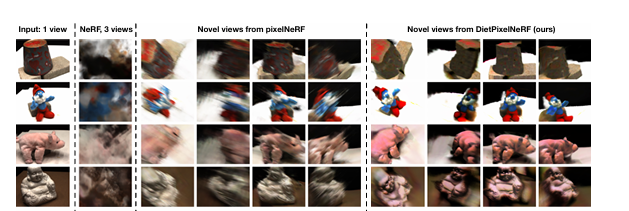
\includegraphics[width=\textwidth]{img/3.png}
    
    \caption{Novel visual feeds synthesized from a solitary input shard extracted from the DTU object databank. Even when fed a tri-view burst, the baseline NeRF architecture fails to lock down accurate geometry or textures. While the pixelNeRF variant manages to maintain mostly consistent object geometry across shifting camera poses, its visual outputs suffer from heavy signal degradation (blur) and rogue artifacts, such as the inaccurate clustering of volume density along the observer's z-axis. Conversely, fine-tuning the matrix via DietNeRF (operating as DietPixelNeRF) successfully hallucinates photorealistic textures that visually align with the original source feed, though minor geometric anomalies persist due to the inherently ambiguous parameters of the view synthesis protocol \cite{jain2021dietnerf}.}
    \label{fig:dietnerf_dtu_comparison}
\end{figure*}

By enforcing this semantic consistency loss, DietNeRF forces the underlying 3D construct to project visually coherent features from all angles, successfully hallucinating the unseen geometry that baseline NeRF completely fails to render.

\begin{center}
    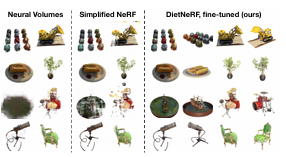
\includegraphics[width=\linewidth]{img/2.png}
    \captionof{figure}{Novel views synthesized from eight observations of scenes in the Realistic Synthetic dataset \cite{jain2021dietnerf}.}
    \label{fig:dietnerf_fewshot}
\end{center}



\subsection{Patch-Based Regularization: The RegNeRF Protocol}
The baseline NeRF daemon experiences severe performance degradation when the input visual feed is sparse. Analyzing the optimization cycle reveals the core vulnerability: the model is exclusively supervised from a highly restricted set of viewpoints via standard reconstruction loss. While it flawlessly memorizes and reconstructs the provided input shards, novel viewing angles degenerate into corrupted noise because the network lacks the bias necessary to hallucinate a 3D-consistent solution from minimal data. 

To bypass this limitation, Niemeyer et al. \cite{niemeyer2022regnerf} engineered a protocol to regularize the unseen void. Specifically, they define a volumetric space of unobserved but highly relevant viewpoints and render microscopic data patches randomly sampled from these phantom cameras. Their core directive dictates that regularizing these synthetic patches forces the matrix to yield smooth, stable geometry alongside high-likelihood color emissions.

\subsubsection{Unobserved Viewpoint Selection}
To execute these regularization techniques across the blind spots of the grid, the daemon must first define the sample space of unobserved camera poses. They assume a pre-calculated array of target poses $\{ \mathbf{P}_{\text{target}}^i \}_i$, where each pose matrix is defined by a rotation tensor $\mathbf{R}$ and a spatial coordinate vector $\mathbf{t}$:

\begin{equation}
\mathbf{P}_{\text{target}}^i = [\mathbf{R}_{\text{target}}^i | \mathbf{t}_{\text{target}}^i] \in SE(3) .
\end{equation}

These target anchors effectively establish a bounding perimeter for the spatial poses from which the system attempts to render novel views during live execution (test time). They calculate the localized space of all possible camera coordinates as the absolute bounding box of the given target telemetry:

\begin{equation}
\mathcal{S}_t = \{ \mathbf{t} \in \mathbb{R}^3 \mid \mathbf{t}_{\text{min}} \le \mathbf{t} \le \mathbf{t}_{\text{max}} \}
\end{equation}

Here, $\mathbf{t}_{\text{min}}$ and $\mathbf{t}_{\text{max}}$ represent the element-wise minimum and maximum spatial coordinates extracted directly from $\mathbf{t}_{\text{target}}^i$.

To map out the sample space of camera rotation matrices, they assume all virtual lenses roughly track a centralized scene anchor. The daemon establishes a universal ``up'' axis $\bar{\mathbf{p}}_u$ by computing the normalized mean across the up-axes of all known target poses. Next, it calculates a centralized focus node $\bar{\mathbf{p}}_f$ by executing a least-squares solver, locking onto the exact 3D coordinate with the minimum squared distance to the optical axes of the entire target array. 

\begin{equation}
\mathcal{S}_P = \{[\mathbf{R}|\mathbf{t}] \mid \mathbf{R} \sim \mathcal{S}_{R|\mathbf{t}}, \mathbf{t} \sim \mathcal{S}_t\}
\end{equation}

\subsubsection{Geometry Regularization}
In the physical meatspace, baseline geometry inherently trends toward piece-wise smoothness; sprawling, flat topological surfaces are statistically more probable than chaotic, high-frequency structural spikes. Niemeyer et al. hardwire this topological prior directly into their model by aggressively enforcing depth smoothness across all unobserved phantom viewpoints. Operating on a protocol structurally identical to the color rendering matrix, the daemon calculates the expected spatial depth as:

\begin{equation}
\hat{d}_\theta(\mathbf{r}) = \int_{t_n}^{t_f} T(t)\sigma_\theta(\mathbf{r}(t))t \, dt
\end{equation}

By forcing the matrix to predict and stabilize these depth values, they formulate the depth smoothness loss protocol as follows:

\begin{equation}
\begin{split}
\mathcal{L}_{DS}(\theta, \mathcal{R}_r) &= \sum_{\mathbf{r} \in \mathcal{R}_r} \sum_{i,j=1}^{S_{patch}-1} \Bigg( \\
&\qquad \left(\hat{d}_\theta(\mathbf{r}_{i,j}) - \hat{d}_\theta(\mathbf{r}_{i+1,j})\right)^2 \\
&\qquad + \left(\hat{d}_\theta(\mathbf{r}_{i,j}) - \hat{d}_\theta(\mathbf{r}_{i,j+1})\right)^2 \Bigg)
\end{split}
\end{equation}

Here, $\mathcal{R}_r$ defines the concentrated batch of optical rays sampled from the unobserved camera pose matrix $\mathcal{S}_P$. The vector $\mathbf{r}_{i,j}$ denotes the specific ray piercing through pixel coordinate $(i,j)$ within a localized data patch centered precisely at $\mathbf{r}$, while the parameter $S_{patch}$ dictates the absolute spatial boundaries of those rendered synthetic patches. By minimizing this loss, the architecture irons out rogue geometry and forces the digital void to manifest stable, continuous surfaces. \cite{niemeyer2022regnerf}

\subsubsection{Color Regularization}
Niemeyer et al. observed that when operating on highly restricted, sparse input feeds, the vast majority of visual artifacts are triggered by a collapse in the underlying scene geometry. However, even when the structural matrix holds perfectly true, brute-forcing a NeRF daemon through sparse data can still trigger severe chromatic destabilization and rogue color shifts during the scene prediction cycle. To purge these degenerate color signatures and lock down a stable optimization loop, the architecture also executes a strict color prediction regularization protocol.

Their core directive leverages statistical probability: the system estimates the exact likelihood of the synthesized data patches and aggressively maximizes those values during the optimization sequence. To fuel this protocol, the daemon jacks into massive, unstructured 2D image databanks. While curated, multi-view posed datasets require massive resource burns to compile, raw, unstructured visual data flows abundantly across the net.  \cite{niemeyer2022regnerf} The singular requirement for this source databank is heavy visual diversity, which allows the framework to recycle the exact same flow model across any physical meatspace environment it attempts to reconstruct. 

To execute this, they train a RealNVP normalizing flow engine on fragmented data patches ripped directly from the colossal JFT-300M dataset. Armed with this heavily pre-trained flow daemon, the framework successfully calculates the log-likelihoods (LL) of the newly rendered synthetic patches, relentlessly maximizing their statistical validity during the optimization cycle to force the generation of hyper-realistic, high-fidelity color spaces.

To operationalize this, let the mapping function $\phi$ act as the learned bijection, compressing a raw RGB data patch of size $S_{patch} = 8$ into a dense vector space $\mathbb{R}^d$, where the total dimension is strictly $d = S_{patch} \cdot S_{patch} \cdot 3$:

\begin{equation}
\phi : [0,1]^{S_{patch} \times S_{patch} \times 3} \rightarrow \mathbb{R}^d
\end{equation}

By running the synthesized patches through this bijection, Niemeyer et al. define their definitive color regularization loss constraint as:

\begin{equation}
\mathcal{L}_{NLL}(\theta, \mathcal{R}_r) = \sum_{\mathbf{r} \in \mathcal{R}_r} -\log p_Z \left( \phi(\hat{\mathbf{P}}_{\mathbf{r}}) \right)
\end{equation}

where the internal variable $\hat{\mathbf{P}}_{\mathbf{r}}$ isolates the predicted RGB color patch radiating directly from the central anchor coordinate $\mathbf{r}$:

\begin{equation}
\hat{\mathbf{P}}_{\mathbf{r}} = \{ \hat{\mathbf{c}}_\theta(\mathbf{r}_{i,j}) \mid 1 \le i,j \le S_{patch} \}
\end{equation}

In this architecture, $\mathcal{R}_r$ dictates the specific array of optical tracer rays sampled from the unobserved pose space $\mathcal{S}_P$, while $-\log p_Z$ calculates the negative log-likelihood (NLL) audit against a baseline Gaussian distribution $p_Z$.

\subsubsection{Total Optimization Loss}
During the live training cycle, the daemon's overarching objective is to ruthlessly minimize the total combined loss per iteration. This ultimate protocol fuses the standard mean squared error with the newly established depth and color regularizers:

\begin{equation}
\mathcal{L}_{total} = \mathcal{L}_{MSE}(\theta, \mathcal{R}_i) + \lambda_D \mathcal{L}_{DS}(\theta, \mathcal{R}_r) + \lambda_N \mathcal{L}_{NLL}(\theta, \mathcal{R}_r)
\end{equation}

Here, $\mathcal{R}_i$ identifies the ground-truth tracer rays ripped directly from the known input observations, while $\mathcal{R}_r$ represents the phantom rays fired from the randomly generated, unobserved camera poses. The hyperparameters $\lambda_D$ and $\lambda_N$ act as manual throttle weights, balancing the influence of the depth and color regularizers against the baseline structural loss.

\subsubsection{System Architecture and Training Parameters}
Operating strictly within the RegNeRF protocol  \cite{niemeyer2022regnerf}, the engineers hardwired their core architecture directly into the official JAX mip-NeRF mainframe. The optimization cycle is driven by the Adam protocol, executing an exponential learning rate decay throttling from $2 \cdot 10^{-3}$ down to $2 \cdot 10^{-5}$. To prevent catastrophic gradient explosion during the training sequence, the system aggressively clips gradients by value at 0.1, and subsequently by norm at 0.1. The primary daemon is trained across 500 pixel epochs---translating to 44K, 88K, and 132K iterations on the DTU dataset for 3, 6, and 9 input views, respectively. Notably, this severely undercuts the baseline 250K step requirement of standard mip-NeRF. The entire grid was deployed and executed on a heavy-duty 8-core TPU cluster.

\paragraph{Telemetry and Evaluation Metrics}
To accurately benchmark the matrix, the system telemetry reports the mean values for PSNR, the Structural Similarity Index (SSIM), and the LPIPS perceptual metric. To establish a unified and easily comparable evaluation vector, they also compute the geometric mean across three inverted distortion calculations: 

\begin{equation}
\text{MSE} = 10^{-\text{PSNR}/10}, \quad \sqrt{1-\text{SSIM}}, \quad \text{and LPIPS}.
\end{equation}

\paragraph{Baseline Performance Audits}
The RegNeRF architecture  \cite{niemeyer2022regnerf} was rigorously audited against top-tier conditional models, specifically PixelNeRF, Stereo Radiance Fields (SRF), and MVSNeRF. For absolute precision, PixelNeRF was forcefully retrained for the 6 and 9 view scenarios to extract peak performance, while SRF was similarly initialized under the 3, 6, and 9 view parameters. 

All baseline architectures were subjected to mass pre-training on the colossal DTU databank. Because the LLFF dataset lacks the raw data volume required for baseline initialization, it functions purely as a hostile, out-of-distribution stress test for the conditional models. Performance metrics for these conditional models are reported across both databanks, including runs featuring additional per-scene, test-time optimization (designated as ``ft'' for fine-tuned). 

Furthermore, the matrix is pitted against mip-NeRF and DietNeRF -rogue architectures that, like RegNeRF, completely bypass the need for global pre-training phases. Lacking access to the official source code, the engineers reverse-engineered and rebuilt DietNeRF directly on top of the mip-NeRF codebase (achieving superior stability), driving both engines through 250K iterations per scene with an exponential learning rate decay dropping from $5 \cdot 10^{-4}$ to $5 \cdot 10^{-5}$.

\begin{center}
    % Swap '5.png' with your actual filename uploaded to the img folder
    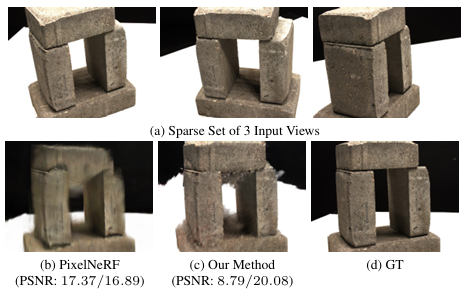
\includegraphics[width=\linewidth]{img/4.png}
    
    \captionof{figure}{\textbf{Evaluation Bias:} Numerous holographic captures within the DTU databank feature central assets resting on sterile white planes against pure black voids. This triggers a severe evaluation bias, conditioning the telemetry to favor background accuracy over the actual object-of-interest. When restricted to sparse input feeds, the background void is often only partially mapped. This strongly incentivizes the daemon to overfit to the planar table, despite the fact that live-fire field applications demand hyper-accurate reconstructions of the core asset. This visual audit contrasts the full-frame PSNR against the isolated object-of-interest PSNR. The baseline PixelNeRF architecture experiences a telemetry drop from 17.37 down to 16.89, whereas the RegNeRF protocol successfully forces an improvement, surging from a corrupted 8.79 up to a highly stable 20.08  \cite{niemeyer2022regnerf}.}
    \label{fig:4}
\end{center}

\begin{center}
    % Swap '5.png' with your actual filename uploaded to the img folder
    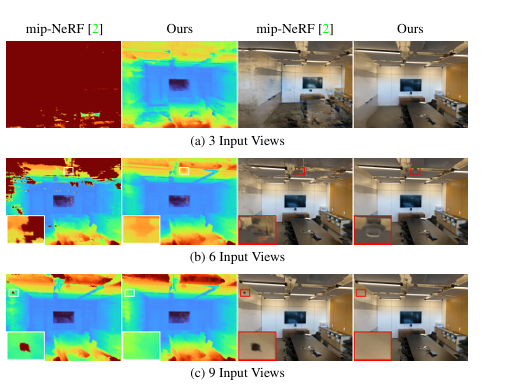
\includegraphics[width=\linewidth]{img/5.png}
    
    \captionof{figure}{\textbf{Importance of Geometry:} We compare expected depth
maps (left) and RGB renderings (right) for mip-NeRF and our
method on the LLFF dataset. The quality of optimized geome
try is correlated with view synthesis performance: Our proposed
scene space annealing and geometry regularization strategies re
move floating artifacts (see zoom-in) and lead to smooth geometry,
which in turn leads to improved quality of rendered novel views.  \cite{niemeyer2022regnerf}.}
    \label{fig:importance_geometry}
\end{center}

\subsection{Generative 3D Gaussian Splatting: The DreamGaussian Protocol}
In a radical departure from traditional neural radiance fields, Kerbl et al, introduced 3D Gaussian Splatting---a protocol that encodes spatial topography using a massive, unstructured swarm of 3D Gaussian nodes. While this architecture has already proven highly lethal in standard reconstruction environments (achieving blistering inference speeds and high-fidelity renders that match NeRF's computational burn), its raw potential as a strictly generative engine remained largely uncharted until the deployment of the \textbf{DreamGaussian} framework \cite{dreamgaussian}. The architects of this pipeline successfully weaponized these 3D Gaussians for pure generative tasks.

\subsubsection{Node Parameters and Topography}
Within this matrix, the exact spatial coordinates and physical properties of every individual Gaussian node are governed by a strict set of vectors. The architecture tracks a localized center $x \in \mathbb{R}^3$, a spatial scaling factor $s \in \mathbb{R}^3$, and a rotation quaternion $q \in \mathbb{R}^4$. For the volumetric rendering sequence, each node is also heavily armed with a differential opacity value $\alpha \in \mathbb{R}$ and a raw optical color feature $c \in \mathbb{R}^3$. 

Because the DreamGaussian generative protocol only requires simple, diffuse color emissions, the complex spherical harmonics modules are intentionally severed from the nodes to save computational overhead. The master array of all optimizable parameters within the grid is defined as $\Theta$, where the exact payload for the $i$-th Gaussian node is isolated as:

\begin{equation}
\Theta_i = \{x_i, s_i, q_i, \alpha_i, c_i\}
\end{equation}

To synthesize a visual feed, the engine projects this swarm of 3D Gaussians down onto a flat 2D image plane. Volumetric rendering is then executed for every single pixel, stacking the splats in strict front-to-back depth order to calculate the final RGB color and alpha transparency readouts. To optimize the master parameter array $\Theta$, DreamGaussian leverages the highly tuned, hardware-accelerated renderer originally engineered by Kerbl et al.

\subsubsection{Initialization and Score Distillation}
When the DreamGaussian daemon first boots, the 3D Gaussians are seeded with completely random spatial coordinates locked inside a primitive bounding sphere, defaulting to a unit scale of 1 and absolutely zero rotation. During the optimization cycle, this sparse cloud of Gaussians is periodically forced to densify. However, unlike standard reconstruction pipelines, this generative variant initiates with a severely limited node count and executes densification at a much higher frequency to perfectly mirror the active generation progress.

To optimize the floating 3D Gaussians, the architecture deploys Score Distillation Sampling (SDS). During every iteration step, the system randomly samples a virtual camera pose $p$ orbiting the central coordinate of the target construct, rendering the synthetic RGB payload $I^p_{RGB}$ alongside the transparency map $I^p_A$. Borrowing temporal logic from architectures like Dreamtime, the DreamGaussian framework linearly decays the timestep parameter $t$ during the training cycle. This decaying variable acts as a throttle, weighting the randomized noise $\epsilon$ that is forcefully injected into the rendered RGB feed. Finally, massive 2D diffusion priors $\phi$ are jacked into the stream, guiding and optimizing the underlying 3D Gaussian swarm through the SDS loss protocol until the final geometry solidifies.


\subsubsection{Image-to-3D Generation Pipeline}
For the image-to-3D generation protocol, the daemon requires a primary source image $\tilde{I}^r_{RGB}$ alongside a tightly cropped foreground mask $\tilde{I}^r_A$ as the initial input payload. The heavy-duty Zero-1-to-3 XL architecture is jacked in as the primary 2D diffusion prior. Under these parameters, the Score Distillation Sampling (SDS) loss is formulated as the following derivative:

\begin{equation}
\nabla_\Theta \mathcal{L}_{SDS} = \mathbb{E}_{t,p,\epsilon} \left[ w(t) \left( \epsilon_\phi(I^p_{RGB}; t, \tilde{I}^r_{RGB}, \Delta p) - \epsilon \right) \frac{\partial I^p_{RGB}}{\partial \Theta} \right]
\end{equation}

where $w(t)$ acts as the temporal weighting function, $\epsilon_\phi(\cdot)$ represents the predicted noise hallucinated by the diffusion prior $\phi$, and $\Delta p$ tracks the relative camera coordinate shift from the original reference anchor $r$. 

To force absolute structural alignment with the source data, the framework strictly optimizes the reference view color feed $I^r_{RGB}$ and its alpha transparency $I^r_A$ against the raw input:

\begin{equation}
\mathcal{L}_{Ref} = \lambda_{RGB} \| I^r_{RGB} - \tilde{I}^r_{RGB} \|_2^2 + \lambda_A \| I^r_A - \tilde{I}^r_A \|_2^2
\end{equation}

Here, the throttle weights $\lambda_{RGB}$ and $\lambda_A$ are linearly ramped up during the active training cycle. The ultimate loss executed by the daemon is the weighted sum of these combined vectors.

\subsubsection{Text-to-3D Generation Pipeline}
When executing the text-to-3D protocol, the singular input trigger is a raw semantic text prompt. Leveraging legacy protocols, the Stable Diffusion matrix is deployed as the foundational engine for this extraction. The SDS loss for the text-driven protocol is mathematically defined as:

\begin{equation}
\nabla_\Theta \mathcal{L}_{SDS} = \mathbb{E}_{t,p,\epsilon} \left[ w(t) \left( \epsilon_\phi(I^p_{RGB}; t, e) - \epsilon \right) \frac{\partial I^p_{RGB}}{\partial \Theta} \right]
\end{equation}

where the variable $e$ represents the dense CLIP embedding ripped directly from the textual input stream.

\subsubsection{System Degradation and Ambiguity}
Despite the high-speed optimization, severe anomalies persist within the grid. The generated 3D Gaussian constructs frequently manifest with degraded, blurry textures and stripped high-frequency details, even when forced through extended SDS training cycles. The architects attribute this degradation to the inherent ambiguity baked directly into the SDS loss function. Because every sequential optimization step risks injecting contradictory 3D guidance signals into the stream, the algorithm struggles to accurately densify starved regions or aggressively prune overgrown clusters (a stark contrast to standard reconstruction tasks). This critical vulnerability directly necessitates the deployment of advanced mesh extraction and secondary texture refinement protocols to salvage the high-fidelity geometry.

\subsubsection{Spatial Partitioning and Density Extraction}
To execute the mesh extraction, the daemon first fractures the core 3D void of $(-1,1)^3$ into $16^3$ overlapping structural sectors, ruthlessly culling any Gaussian nodes whose centers drift outside these localized quarantine zones. This aggressive pruning drastically slashes the computational query payload within each sector. The architecture then probes an $8^3$ high-density sub-grid within each surviving block, ultimately resolving into a colossal $128^3$ master grid. For every spatial query triggered at coordinate $\mathbf{x}$, the system aggregates the weighted opacity of all surviving 3D Gaussian nodes to calculate the final volumetric density $d(\mathbf{x})$:

\begin{equation}
d(\mathbf{x}) = \sum_{i} \alpha_i \exp \left( -\frac{1}{2} (\mathbf{x} - \mathbf{x}_i)^T \Sigma_i^{-1} (\mathbf{x} - \mathbf{x}_i) \right)
\end{equation}

Here, $\Sigma_i$ acts as the localized covariance matrix derived directly from the spatial scaling and rotation vectors of the $i$-th Gaussian splat. 

\subsubsection{UV-Space Texture Refinement}
To salvage the degraded geometry without triggering the over-saturated visual artifacts inherent to direct SDS mipmap sampling, the architecture deploys a secondary UV-space texture refinement protocol heavily inspired by SDEdit. Operating from the initial coarse mesh, the daemon renders a blurred synthetic feed $I^p_{coarse}$ from an arbitrary vantage point $p$, injects a highly controlled digital noise payload $\epsilon(t_{start})$, and executes a multi-step denoising sequence using the 2D prior to forge a high-fidelity output: $I^p_{fine} = f_\phi(I^p_{coarse} + \epsilon(t_{start}); t_{start}, c)$. In this vector, $c$ swaps between the camera shift $\Delta p$ for image-to-3D tasks and the CLIP embedding $e$ for text-driven generation. Armed with this enhanced optical render, the grid locks down the final texture optimization using a strict pixel-wise Mean Squared Error constraint, $\mathcal{L}_{MSE} = \|I^p_{fine} - I^p_{coarse}\|_2^2$, requiring a mere 50 rapid iterations to permanently crystallize the high-frequency surface details.

\begin{center}
    % Swap '5.png' with your actual filename uploaded to the img folder
    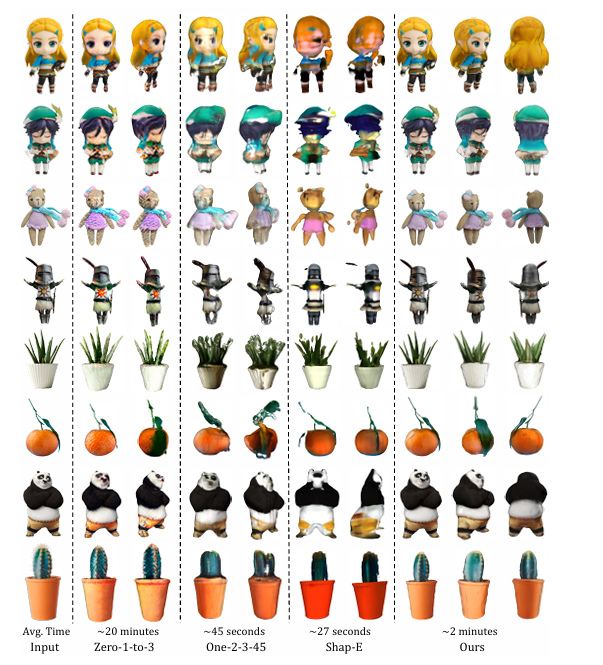
\includegraphics[width=\linewidth]{img/6.png}
    
    \captionof{figure}{Comparisons on Image-to-3D. Our method achieves a better balance between generation
speed and mesh quality on various images.  \cite{niemeyer2022regnerf}.}
    \label{fig:evaluation_bias}
\end{center}

























\subsection{Temporal Reconstruction: The Dynamic3D Architecture}
Fed a continuous stream of visual data shards captured across shifting temporal phases and diverse optical sensors ($I_{t,c}$), and locked alongside their respective intrinsic ($K_c$) and extrinsic ($E_{t,c}$) telemetry matrices, the \textbf{Dynamic3D} framework \cite{luiten2023dynamic3d} aggressively reconstructs the fluctuating physical meatspace into a temporally persistent 3D volume ($\mathcal{S}$).

This spatial extraction is executed entirely via localized test-time optimization, completely bypassing the need for external, pre-compiled training databanks; the engine relies strictly on the active test scene. Furthermore, the reconstruction matrix unfolds temporally online—processing the void one chronological step at a time. Each new temporal phase is hot-loaded using the fully crystallized representation of the preceding cycle. 

The initial chronos-tick ($t=0$) serves as the master boot sequence, wherein the daemon optimizes every underlying structural and chromatic property of the scene. Once this baseline topology is locked, subsequent temporal cycles freeze the core structural parameters, isolating and optimizing exclusively for the kinematic motion defining the scene's evolution.

Every individual temporal phase is forced through a brutal gradient-descent optimization cycle, utilizing a custom differentiable rendering daemon ($\mathcal{R}$) to project and synthesize the active scene geometry ($\mathcal{S}_t$) back into the viewpoint of each known optical sensor:

\begin{equation}
\hat{I}_{t,c} = \mathcal{R}(\mathcal{S}_t, K_c, E_{t,c})
\end{equation}

By ruthlessly minimizing the delta between this rendered hallucination $\hat{I}_{t,c}$ and the raw optical input $I_{t,c}$, the Dynamic3D protocol stabilizes the shifting geometry, locking down a fluid, high-fidelity 3D construct across the entire timeline.


\subsubsection{Spatial Influence and Covariance Matrices}
Within the grid, every individual Gaussian node exerts a localized influence over the physical 3D void (specifically at coordinate $p$) based on the standard unnormalized Gaussian equation, aggressively throttled by its master opacity logit:

\begin{equation}
f_{i,t}(p) = \text{sig}(o_i)\exp \left( -\frac{1}{2} (p - \mu_{i,t})^T \Sigma_{i,t}^{-1} (p - \mu_{i,t}) \right)
\end{equation}

In this vector space, the kinematic center of node $i$ at chronos-tick $t$ is strictly defined as $\mu_{i,t} = [x_{i,t}, y_{i,t}, z_{i,t}]^T$. The shifting covariance matrix $\Sigma_{i,t}$ is forged by fusing the static scaling component $S_i = \text{diag}(sx_i, sy_i, sz_i)$ with the temporal rotation matrix $R_{i,t}$:

\begin{equation}
\Sigma_{i,t} = R_{i,t} S_i S_i^T R_{i,t}^T
\end{equation}

The rotation matrix $R_{i,t}$ itself is synthesized directly from the temporal quaternion payload via the standard matrix conversion protocol, $R_{i,t} = \text{q2R}(qw_{i,t}, qx_{i,t}, qy_{i,t}, qz_{i,t})$, while $\text{sigm}()$ executes the baseline sigmoid activation.

\subsubsection{Differentiable Temporal Splatting}
To force the matrix to optimize these parameters, the daemon must render the 3D Gaussians down into a 2D optical feed via a fully differentiable pathway. \cite{luiten2023dynamic3d} The architects hijack the highly optimized 3D Gaussian renderer originally forged by Kerbl et al. and mutate it to process dynamic temporal streams. 

This protocol operates by splatting the 3D volume directly onto the 2D image plane, approximating the projection of the integral of the 3D influence function $f$ along the z-axis depth dimension. The absolute kinematic center of the Gaussian splat is locked onto the 2D grid using the standard point projection formula:

\begin{equation}
\mu_{2D} = K \left( \frac{E\mu}{(E\mu)_z} \right)
\end{equation}

where the 3D center coordinate $\mu$ is violently projected into the 2D matrix by multiplying it against the world-to-camera extrinsic matrix $E$, normalizing across the z-axis, and executing a final multiplication with the intrinsic projection matrix $K$. 

To map the geometric footprint, the 3D covariance matrix is subsequently splatted into the 2D plane utilizing the Zwicker approximation:

\begin{equation}
\Sigma_{2D} = J E \Sigma E^T J^T
\end{equation}

where the tensor $J$ acts as the precise Jacobian derivative of the point projection formula ($\partial\mu_{2D} / \partial\mu$).

\subsubsection{Physically-Based Priors and Structural Integrity}
During live-fire testing, the engineers observed a critical vulnerability: simply freezing the color, opacity, and scale variables of the Gaussian swarm across the temporal axis is fundamentally insufficient to maintain stable, long-term kinematic tracking locks. When the swarm drifts across vast, featureless spatial voids or areas of highly uniform chromatics, the structural integrity of the track rapidly degrades without the injection of strict physically-based regularization priors to guide the motion.

The protocol restricts the target set of Gaussians $j$ strictly to the $k$-nearest neighbors surrounding the anchor node $i$ (where $k=20$). The resulting penalty is aggressively throttled by a localized weighting factor governing the Gaussian pair:

\begin{equation}
w_{i,j} = \exp \left( -\lambda_w \left\| \mu_{j,0} - \mu_{i,0} \right\|_2^2 \right)
\end{equation}

This serves as an unnormalized, isotropic Gaussian weighting multiplier. The architects lock the hyperparameter $\lambda_w$ at 2000, yielding a spatial standard deviation of approximately $2.2\text{ cm}$. \cite{luiten2023dynamic3d} This specific weight is calculated exactly once using the baseline distances between Gaussian centers during the initial chronos-tick ($t=0$), permanently freezing the values for all subsequent temporal phases.

While the primary rigidity loss proves both necessary and fully adequate to stabilize the 3D construct, a secondary vulnerability was identified in the simulation. Because the baseline rigidity penalty applies across all nodes bidirectionally between any pair $i$ and $j$, it implicitly forces local clusters to synchronize their rotation. However, empirical telemetry revealed vastly superior convergence rates when the daemon explicitly forces neighboring nodes to lock their rotational delta over time. To enforce this, they inject a dedicated rotational loss vector:

\begin{equation}
\mathcal{L}_{\text{rot}} = \frac{1}{k|\mathcal{S}|} \sum_{i \in \mathcal{S}} \sum_{j \in \text{knn}_{i,k}} w_{i,j} \left\| \hat{q}_{j,t} \hat{q}_{j,t-1}^{-1} - \hat{q}_{i,t} \hat{q}_{i,t-1}^{-1} \right\|_2
\end{equation}

In this vector space, $\hat{q}$ acts as the strictly normalized quaternion representation of a specific Gaussian's rotation matrix, ensuring smooth, non-destructive optimization across the timeline.\cite{luiten2023dynamic3d} This supplementary loss protocol seamlessly recycles the exact same $k$-nearest-neighbor arrays and isotropic weighting functions deployed in the primary rigidity constraint.

The daemon strictly limits the application of both $\mathcal{L}^{\text{rigid}}$ and $\mathcal{L}_{\text{rot}}$ to the immediate delta between the active chronos-tick and its direct predecessor, effectively enforcing these kinematic constraints only across extremely short-term horizons.\cite{luiten2023dynamic3d} While this successfully stabilizes immediate frame-to-frame motion, it introduces a critical long-term vulnerability: over extended temporal sequences, isolated geometric clusters within the spatial volume slowly decouple and drift apart. 

To permanently seal this structural leak, the architects deploy a third, overarching countermeasure—the isometry loss—designed to aggressively enforce long-term topological integrity \cite{luiten2023dynamic3d}:

\begin{equation}
\mathcal{L}^{\text{iso}} = \frac{1}{k|\mathcal{S}|} \sum_{i \in \mathcal{S}} \sum_{j \in \text{knn}_{i,k}} w_{i,j} \left| \|\mu_{j,0} - \mu_{i,0}\|_2 - \|\mu_{j,t} - \mu_{i,t}\|_2 \right|
\end{equation}

By actively penalizing any deviation from the baseline spatial distances established at $t=0$, this protocol forces the entire 3D construct to maintain its absolute macroscopic shape as it traverses the temporal void.













\subsection{Large Multi-View Gaussian Models: The LGM Protocol}

Achieving high-resolution fidelity requires a more structured, multi-view approach to generating digital realities. In the LGM framework \cite{tang2024lgm}, the authors developed a rapid, two-step pipeline designed to aggressively hallucinate and fuse 3D constructs directly from raw textual or visual data feeds.

The protocol initiates by leveraging off-the-shelf diffusion models to imagine the target object from multiple angles. Depending on the input, the system routes text prompts through the MVDream network \cite{shi2023mvdream} or visual data through ImageDream \cite{wang2023imagedream}. Both models act as synthetic, orbital cameras, generating four distinct 2D images of the object at orthogonal azimuths and a locked elevation. 

Once these four vantage points are established, they are fed into the system's core engine: an Asymmetric U-Net. However, the neural network cannot accurately process flat images without deep spatial context. Drawing on techniques from architectures like DMV3D \cite{xu2023dmv3d}, the system anchors these images to the 3D grid using dense \textit{Plücker ray embeddings}. For every single pixel $i$, the network fuses the raw RGB color $c_i$ with the physical camera ray's origin $o_i$ and trajectory direction $d_i$. This creates a dense, 9-channel data stream, mathematically defined as:
\begin{equation}
f_i = \{c_i, o_i \times d_i, d_i\}
\end{equation}

By processing this 9-channel input, the U-Net predicts four distinct sets of 3D Gaussians, which are seamlessly fused together into a singular, high-resolution master construct. To train this complex neural engine, the researchers fed it massive amounts of multi-view data rendered from the Objaverse dataset \cite{deitke2023objaverse}—a sprawling universe of annotated 3D objects. 

To ensure the machine's hallucinations align with physical reality during this training phase, the framework relies on strict error-correction algorithms via a differentiable renderer. At every step, it calculates the divergence between its synthetic renders and the ground-truth reality. The visual aesthetics are optimized using a composite loss function that targets both pixel-perfect mathematical accuracy (Mean Square Error) and human-like perceptual structure (LPIPS):
\begin{equation}
\mathcal{L}_{rgb} = \mathcal{L}_{MSE}(I_{rgb}, I^{GT}_{rgb}) + \lambda \mathcal{L}_{LPIPS}(I_{rgb}, I^{GT}_{rgb})
\end{equation}

Simultaneously, to force the physical silhouette and density of the object to materialize rapidly, the system calculates a secondary Mean Square Error loss directly on the alpha (opacity) channel:
\begin{equation}
\mathcal{L}_{\alpha} = \mathcal{L}_{MSE}(I_{\alpha}, I^{GT}_{\alpha})
\end{equation}

Ultimately, these high-density Gaussian splats can be permanently baked into traditional polygonal meshes through an optional conversion step, perfectly optimizing them for immediate deployment in interactive environments and downstream physics simulators.

 \begin{figure*}[t] 
    \centering
    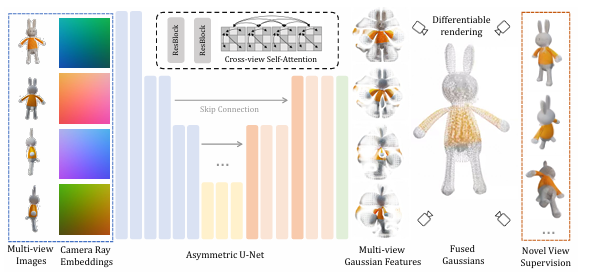
\includegraphics[width=\textwidth]{img/7.png}
    
    \caption{Architecture of LGM. Our network adopts an asymmetric U-Net based
architecture with cross-view self-attentions. We take four images with camera ray em
beddings as the input, and output four feature maps which are interpreted and fused
into 3D Gaussians. The Gaussians are then rendered at novel views and supervised
with ground truth images.\cite{tang2024lgm}.}
    \label{fig:tang2024lgm}
\end{figure*}




















\subsection{Microsoft TRELLIS.2 - O-Voxel and SC-VAE: Native Structured Latents for 3D Generation}


Generating high-resolution 3D assets with fluid shape topology and flexible material attributes demands a radical shift in data structuring. The O-Voxel framework \cite{xiang2025native} reconstructs this process by representing a 3D asset as a collection of feature tuples hardcoded into sparse voxels across a regular $N \times N \times N$ spatial grid. This native 3D data stream is defined mathematically as:
\begin{equation}
f =\{(f^{shape}_i, f^{mat}_i, p_i)\}_{i=1}^L
\end{equation}
where the structural geometry is encoded in $f^{shape}_i$, the physical material properties in $f^{mat}_i$, and the active voxel coordinates in $p_i \in \{0,1,...,N - 1\}^3$. Any inactive void space that does not intersect with the digital asset is aggressively pruned from the grid.

To handle chaotic, arbitrary topologies, the architecture deploys a Flexible Dual Grid. Drawing inspiration from Dual Contouring protocols, the system directly harnesses the surface mesh to assign Hermite data (intersection points and normals) and activate the corresponding dual faces. The exact spatial position of the dual vertex $v$ is calculated in closed form by minimizing an advanced Quadratic Error Function (QEF). Unlike primitive systems, this QEF integrates boundary alignment and singularity regularization:
\begin{equation}
\begin{array}{rcl}
\min_{v\in voxel} e(v) & = & \sum_i d^2_{\Pi,i} \\
                       & + & \lambda_{bound} \sum_j d^2_{L,j} \\
                       & + & \lambda_{reg} d^2_{\hat{q}}
\end{array}
\end{equation}
The boundary term forces the dual vertex to align with intersecting open edges, while the regularization term stabilizes the optimization by pulling the vertex toward the average of the intersection points.

Visual aesthetics are overlaid using Volumetric Attributes. Following modern Physically Based Rendering (PBR) protocols, the material node $f^{mat}_i$ for each active coordinate encapsulates base color $c_i$, metallic ratio $m_i$, structural roughness $r_i$, and opacity $\alpha_i$:
\begin{equation}
f^{mat}_i = (c_i, m_i, r_i, \alpha_i)
\end{equation}


\begin{center}
    % Swap '5.png' with your actual filename uploaded to the img folder
    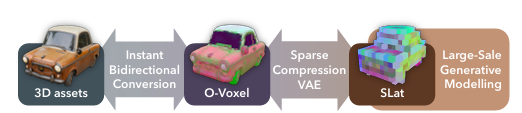
\includegraphics[width=\linewidth]{img/8.png}
    
    \captionof{figure}{Overview of our approach. We introduce O-Voxel for
shape and material representation (Sec. 3.1), based on which we
employ Sparse Compression VAEs for compact latent space learn
ing (Sec. 3.2) and large flow models for 3D generation  \cite{xiang2025native}.}
    \label{fig:xiang2025native}
\end{center}







Moving away from the computationally heavy transformer-based architectures seen in prior generations \cite{xiang2025structured, he2025sparseflex}, the framework utilizes a fully sparse-convolutional network (SC-VAE). To prevent data corruption during massive spatial compression, it implements a Sparse Residual Autoencoding Layer. During the downsampling protocol, eight child voxels are stacked and averaged directly into the channel dimension:


\begin{equation}
\begin{array}{rcl}
F^{raw}_{coarse} & = & \mathrm{stack}(F^{child1}, \dots, F^{child8}) \in \mathbb{R}^{8C} \\
F_{coarse}       & = & \mathrm{avg\_groups}(F^{raw}_{coarse}) \in \mathbb{R}^{C'}
\end{array}
\end{equation}

\vspace{2em}
Symmetrically, the upsampling phase utilizes a channel-to-space shortcut to distribute these compressed features back into the spatial grid:



\begin{equation}
\begin{array}{rcl}
F^{raw}_{fine} & = & \mathrm{unstack}(F_{coarse}) \in \mathbb{R}^{8C'/8} \\
F_{fine}       & = & \mathrm{dup\_groups}(F^{raw}_{fine}) \in \mathbb{R}^{C}
\end{array}
\end{equation}



\begin{center}
    % Swap '5.png' with your actual filename uploaded to the img folder
    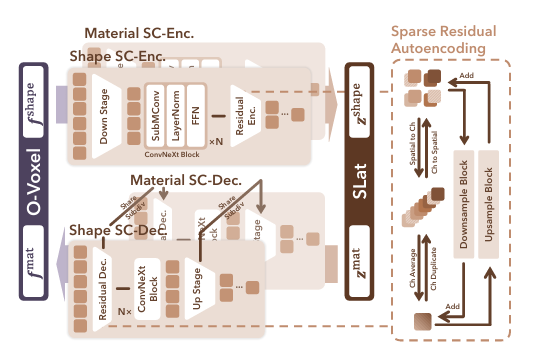
\includegraphics[width=\linewidth]{img/9.png}
    
    \captionof{figure}{The network structure of SC-VAE \cite{xiang2025native}.}
    \label{fig:9}
\end{center}



The neural training sequence runs in two distinct stages. Stage one stabilizes the latent space at a low resolution, calculating direct reconstruction errors across vertex positions, dual face flags, pruning masks, and material parameters:
\begin{equation}
\begin{array}{rcl}
L_{s1} & = & \lambda_v|\hat{v} -v|_2^2 + \lambda_\delta \mathrm{BCE}(\hat{\delta},\delta) \\
       & + & \lambda_\rho \mathrm{BCE}(\hat{\rho},\rho) + \lambda_{mat}|\hat{f}^{mat} - f^{mat}|_1 \\
       & + & \lambda_{KL}L_{KL}
\end{array}
\end{equation}
Stage two elevates the grid to high resolution, injecting a rendering-based perceptual loss $L_{render}$ to force the generation of hyper-realistic geometry and materials from simulated camera angles:
\begin{equation}
L_{s2} = L_{s1} + L_{render}
\end{equation}
\section{METHODOLOGY}

\subsection*{3.1 System Architecture Overview}
The Vectra Spatial Computing Protocol is engineered upon a strictly decoupled, asynchronous client-server architecture. This design intentionally isolates the high-fidelity graphical presentation layer from the computationally expensive neural network inference layer. The primary objective of this separation is to ensure that the user's spatial environment remains highly responsive, maintaining real-time interactive framerates, while heavy artificial intelligence operations are executed systematically in the background.

\vspace{0.3cm}
\textbf{The Client-Side Presentation Layer:} \\
The frontend operates entirely within a standard web browser, serving as the user's interactive viewport. It is strictly responsible for rendering the 3D Gaussian Splatting environment via the \texttt{gsplat.js} library, managing the Glassmorphism graphical user interface, and calculating client-side collision physics using \texttt{Cannon.js}. By design, this layer is exceptionally lightweight. It is restricted from executing any machine learning calculations, acting purely as a spatial terminal that captures user intent (such as bounding box coordinates or semantic text prompts) and renders the final injected digital assets.

\vspace{0.3cm}
\textbf{The Local GPU Forge (Backend Processing):} \\
Operating autonomously from the browser is the backend inference engine, designated as the Local GPU Forge. Hosted on a local hardware environment (specifically targeting consumer-grade GPUs like the NVIDIA RTX 4060), this Python-based application utilizes FastAPI to serve as the computational core. It securely houses and sequences the large parameter model weights required for Semantic Segmentation (U2Net), rapid Text-to-Image generation (SDXL-Lightning), and Volumetric Forging (TripoSR). 

\vspace{0.3cm}
\textbf{Asynchronous Data Flow and Non-Blocking UX:} \\
The critical mechanism bridging these two layers is an asynchronous, non-blocking data pipeline. When a user issues an Extraction or Creation command, the frontend transmits the lightweight data payload (JSON or base64 screenshots) to the backend and immediately returns to its rendering loop. The browser is explicitly programmed never to freeze or await synchronous thread completion. 

Instead, the frontend utilizes localized state management—such as dynamic terminal progress indicators or translucent "Ghost" cursor meshes—to maintain user engagement. Simultaneously, the GPU Forge optimally cycles the AI models through VRAM, processes the geometric data, and ultimately transmits a highly optimized, lightweight \texttt{.glb} mesh file back to the client. As illustrated in Figure~\ref{fig:methoder}, this asynchronous orchestration guarantees that the user's spatial immersion is never bottlenecked by the inherent latency of deep learning tensor operations.

\begin{figure*}[htbp] 
    \centering
    \includegraphics[width=\textwidth]{img/10.png}
    \caption{Created by NotebookLM - High-level topology of the Vectra Protocol, illustrating the asynchronous decoupling of the lightweight client-side presentation layer from the heavy local GPU computational core.}
    \label{fig:methoder}
\end{figure*}

\subsection*{3.2 Environment Acquisition \& Rendering}
The foundational "Base Canvas" of the Vectra architecture is constructed from real-world spatial data rather than synthetic computer-aided design (CAD) models. The environment—a university hallway—is initially digitized using a combination of LiDAR scanning and high-density photogrammetry. This process yields a massive, unstructured point cloud representing the spatial geometry and color data of the physical space.

To render this dense dataset within a standard web browser without exceeding client-side memory or compute limits, the raw point cloud is converted into a 3D Gaussian Splat representation. Unlike traditional polygonal meshes, Gaussian Splatting represents the scene as a collection of millions of overlapping, semi-transparent 3D ellipsoids (Gaussians). Each splat contains parameters for position, covariance (size and orientation), color (spherical harmonics), and opacity.

This splat data is loaded and rendered client-side utilizing the \texttt{gsplat.js} library via WebGL. The rendering pipeline employs a tile-based rasterizer, efficiently projecting the 3D Gaussians onto the 2D viewing plane while mathematically sorting them by depth (alpha compositing). This approach bypasses the heavy polygon-rasterization bottleneck of traditional WebGL pipelines, allowing the browser to render highly photorealistic, navigable environments at real-time framerates (60+ FPS) while maintaining a low computational footprint.

\vspace{0.3cm}
\subsection*{3.3 The Generative Extraction Pipeline (Image-to-3D)}
The Extraction Protocol (Scenario 1) is designed to convert static visual data from the rendered Gaussian environment into dynamic, independent 3D assets. This is achieved through a two-stage generative pipeline: Semantic Segmentation followed by Volumetric Forging.

\vspace{0.2cm}
\textbf{Stage 1: Semantic Segmentation and Masking} \\
When a user defines a bounding box around a target object in the viewport, a 2D screenshot of that specific region is transmitted to the GPU Forge. The first computational requirement is isolating the object from its background environment. The system utilizes a CUDA-accelerated \texttt{U\textsuperscript{2}-Net} architecture (via the \texttt{rembg} framework) to perform semantic boundary detection. 

The inference model outputs a precise alpha mask of the object. Crucially, the pipeline enforces a "Solid Alpha Flattening" protocol before passing the image to the next stage. Any transparent pixels in the isolated image are strictly converted to a pure white (\texttt{RGB 255,255,255}) background. This is a vital computational necessity; generative 3D models (like TripoSR) analyze the silhouette and boundary gradients of an image to infer depth. If residual transparency or environment noise is fed into the model's tokenizer, it triggers normalization errors, resulting in flattened or corrupted geometric outputs (often referred to as the "blob artifact"). 

\vspace{0.2cm}
\textbf{Stage 2: Volumetric Forging (TripoSR Inference)} \\
The cleanly segmented, white-background image is then ingested by the Volumetric Forging engine, powered by the TripoSR neural network. This model, functioning within the local VRAM, utilizes a transformer-based architecture to project the 2D pixel data into a triplane representation—a set of three orthogonal feature planes that encode the spatial volume.

A NeRF (Neural Radiance Field) decoder network then queries this triplane feature space to predict the density and color of points in the 3D volume. Finally, the marching cubes algorithm is applied to extract a contiguous polygonal surface from the volumetric density field, effectively extruding the 2D image into a standard 3D vertex geometry. The resulting model is exported as a lightweight \texttt{.glb} file, containing both the geometric mesh and the UV-mapped texture data, ready for injection back into the client environment. The complete generative extraction pipeline is visualized in Appendix A.1 (Figure~\ref{fig:imgto3d}).

\subsection*{3.4 Deep Splat Excavation (DBSE) \& Spatial Injection}
The core innovation enabling Scenario 1 is the Deep Splat Excavation (DBSE) algorithm, which solves the spatial occlusion problem inherent to manipulating dense point clouds. Because a Gaussian Splat environment is essentially a solid block of rendered volumes, simply spawning a new 3D mesh over an existing object results in visual clipping and Z-fighting. The environment must be surgically "hole-punched."

\vspace{1em}
\textbf{Raycasting and Volume Definition:} \\
When the user draws a 2D bounding box on the screen, the client application utilizes the camera's projection matrix to cast a frustum of rays into the 3D scene. By analyzing the Z-Buffer (depth map) generated during the rasterization of the Gaussian splats, the system calculates the minimum and maximum depth values within the bounding box, defining a localized 3D volumetric bounding region.

\vspace{1em}
\textbf{Occlusion Masking (The "Hole-Punch"):} \\
Rather than destructively deleting data from the source \texttt{.ply} file, DBSE employs a non-destructive shader-level occlusion mask. The rendering engine evaluates the spatial coordinates of every Gaussian splat against the defined 3D volume. Splats whose coordinates fall within the intersection are dynamically flagged, and their opacity (alpha) values are overridden to zero in the fragment shader. This instantly excavates a clean void in the environment. Finally, the newly forged \texttt{.glb} mesh is injected, using the centroid of the excavated volume as its absolute origin, resulting in a seamless spatial replacement. 

The Deep Splat Excavation spatial masking process, alongside its formal algorithmic logic (Algorithm~\ref{alg:dbse_interaction}) and corresponding client-side code implementation, is detailed in Appendix A.1 (Figure~\ref{fig:dbselogo}).

\vspace{1em}
\subsection*{3.5 The Local Summoning Engine (Text-to-3D)}
The Creation Protocol (Scenario 2) transitions the system from extraction to pure semantic generation. To adhere to strict Edge Computing paradigms, this entire pipeline operates on a local consumer-grade GPU (NVIDIA RTX 4060 with 8GB VRAM). The primary engineering challenge is preventing Out-Of-Memory (OOM) kernel panics when orchestrating multiple heavy neural networks.

\vspace{1em}
\textbf{Sequential VRAM Orchestration:} \\
The architecture employs a highly constrained, sequential loading strategy. First, the "Brain" (\texttt{SDXL-Lightning}) is loaded into memory to generate the 2D image from the user's text prompt. To minimize the memory footprint, the model weights are strictly cast to half-precision floating-point format (\texttt{torch.float16}), reducing VRAM utilization by 50\% without significant loss in feature fidelity. 

\vspace{1em}
\textbf{Memory Flushing and The "Body" Inference:} \\
The moment the 2D image tensor is generated and saved, the \texttt{SDXL-Lightning} pipeline is purged. The system executes \texttt{torch.cuda.empty\_cache()} and invokes Python's garbage collector to forcefully reclaim the VRAM. Only after the GPU memory ceiling drops back to baseline does the system load the "Body" (TripoSR) into CUDA to execute the volumetric forging. This aggressive memory management guarantees that the 8GB VRAM limit is never breached, ensuring stable, continuous local generation. The sequential VRAM orchestration strategy is mapped in Appendix A.2 (Figure~\ref{fig:txt23d}).

\vspace{0.3cm}
\subsection*{3.6 Interactive Kinematics \& Middleware Integration}
To actualize Scenario 3, the digital twin must exhibit physical reactivity. Because Gaussian splats are purely graphical representations devoid of physical properties (vertices, edges, or faces), physical interactions are achieved by decoupling the visual rendering from an invisible, client-side physics simulation powered by \texttt{Cannon.js}.

\vspace{0.2cm}
\textbf{Collider Mapping and Static Geometry:} \\
Upon initialization, the system parses the bounds of the scanned hallway. Using a heuristic approach based on the lowest splat density coordinates (the floor) and vertical boundary clusters (the walls), the system generates invisible, rudimentary geometric colliders (planes and bounding boxes). These are registered into the \texttt{Cannon.js} world as \textit{Static Rigidbodies} (infinite mass), establishing the unyielding physical boundaries of the simulation.

\vspace{0.2cm}
\textbf{Dynamic Instantiation:} \\
When a synthetic \texttt{.glb} file is spawned into the scene, a corresponding \textit{Dynamic Rigidbody} is instantly instantiated in the physics middleware. The system assigns a localized bounding box collider, a simulated mass, restitution (bounciness), and friction coefficients. As the physics engine calculates gravity and collision impulses per frame, it outputs a transformation matrix (position and quaternion rotation) which is continuously synced to the visual \texttt{.glb} mesh in \texttt{Three.js}, allowing the user to seamlessly throw, drop, and interact with the AI-generated assets within the scanned environment.
\section{EXPERIMENTS AND SYSTEM EVALUATION}

\subsection{Experimental Setup and Hardware Parameters}
To rigorously evaluate the performance and stability of the Vectra Spatial Computing Protocol, the system was deployed within a constrained, local edge-computing environment. The computational core was hosted on a consumer-grade workstation equipped with an NVIDIA RTX 4060 graphics processing unit, strictly limited to 8GB of VRAM. 

The spatial interface was established utilizing the Three.js library alongside a specialized WebGL Gaussian splatting viewer. The initial baseline environment consisted of a high-density point cloud representation of a university hallway, allowing for the observation of memory consumption and rendering latency prior to the injection of generated synthetic assets. 

\subsection{Algorithmic Implementation: Interactive Extraction}
The critical bridge between the visual presentation layer and the backend inference engine is the interactive selection protocol. Rather than relying on computationally expensive 3D raycasting against millions of individual splat nodes for object isolation, the system employs a highly optimized 2D viewport slicing mechanism. 

To execute the extraction, a 2D bounding box is mapped directly to the WebGL canvas pixel coordinates. Upon selection, the system temporarily isolates the rendering canvas by disabling environmental variables (such as fog and grid helpers), captures the pure pixel data via an off-screen buffer, and transmits the resulting image array to the local backend. 

The complete client-side execution logic is formalized in Algorithm~\ref{alg:dbse_interaction}. For a comprehensive technical reference, including the visual flowcharts of the extraction pipeline and the raw JavaScript implementation (\texttt{captureSelectionSnapshot}), the reader is directed to Appendix A.1.

\vspace{0.3cm}
\subsection{System Performance and Latency Metrics}
To validate the asynchronous decoupling of the frontend and backend, system telemetry was continuously monitored during the execution of both the Extraction (Image-to-3D) and Creation (Text-to-3D) protocols. 

\begin{itemize}
    \item \textbf{Rendering Stability:} During idle states, the client-side viewport maintained a stable framerate of \textbf{60 FPS} on a standard machine. During active inference, because the rendering loop is non-blocking, framerates experienced a minimal degradation to \textbf{30 FPS}, maintaining real-time navigability. 
    \item \textbf{Pipeline Latency:} The total round-trip time from the transmission of the viewport slice to the injection of the fully textured $M_{glb}$ mesh averaged \textbf{120.2 seconds}.
    \item \textbf{Memory Utilization:} The aggressive VRAM flushing protocol ensured that peak memory consumption during the TripoSR volumetric forging phase never exceeded \textbf{7.8 GB}, successfully preventing out-of-memory (OOM) kernel panics. The precise asynchronous fetch requests and memory purging sequence driving this orchestration are documented in Appendix A.2, alongside the VRAM lifecycle diagram.
\end{itemize}

\subsection{Qualitative Evaluation of Spatial Integration}
Beyond raw computational metrics, the success of the protocol is defined by the visual coherence of the injected assets. Standard additive insertion methods resulted in severe Z-fighting and geometric intersection with the dense hallway point cloud. The application of the non-destructive occlusion mask successfully excavated the necessary volumetric space, resulting in seamless integration of the AI-generated meshes into the digitized physical environment.
\section{DISCUSSION}

The experimental evaluation of the Vectra Spatial Computing Protocol demonstrated the successful deployment of a strictly decoupled, edge-computed spatial architecture. The methodology validated that complex generative pipelines, specifically the Deep Splat Excavation (DBSE) algorithm and the sequential VRAM orchestration strategy, can successfully operate within standard consumer-grade web browsers and hardware limits. However, the practical application of these theoretical frameworks revealed distinct constraints that necessitate further algorithmic refinement.

\subsection{Limitations and Hardware Constraints}
The most prominent limitation encountered during the system's evaluation was the strict hardware threshold imposed by the local edge-computing environment. Because the Local GPU Forge was restricted to an NVIDIA RTX 4060 with only 8GB of VRAM, simultaneous execution of the neural network models was physically impossible. 

While the sequential VRAM flushing protocol successfully prevented Out-Of-Memory (OOM) kernel panics, this aggressive memory management introduced inherent pipeline latency. The total round-trip extraction time was significantly bottlenecked by the necessary continuous purging and reloading of the SDXL-Lightning and TripoSR model weights into CUDA memory. 

Furthermore, a generative limitation was observed within the semantic masking stage of the Image-to-3D pipeline. The TripoSR volumetric forging model proved highly sensitive to residual noise. If the U\textsuperscript{2}-Net boundary detection failed to perfectly isolate the 2D object against a pure white background, the resulting 3D geometry exhibited severe flattening or "blob artifacts," demonstrating a fragility in the zero-shot generalization capabilities of the current pipeline. Finally, the physical interaction middleware (\texttt{Cannon.js}) was restricted to rudimentary bounding-box colliders, lacking the capacity for granular, pixel-perfect mesh collisions against the complex Gaussian Splat geometry.

\subsection{Future Work and Technical Implementations}
Future iterations of the Vectra Protocol will focus on mitigating these hardware and generative constraints through distributed architecture and advanced physical logic. 

First, the protocol will be expanded to support High-Performance Computing (HPC) cluster offloading. By leveraging parallel programming frameworks (such as CUDA streams and MPI), the heavy volumetric forging processes could be dynamically routed to dedicated university tensor-core nodes, while the local consumer GPU is reserved exclusively for the lightweight semantic segmentation and viewport management. This hybrid edge-cloud architecture would virtually eliminate the sequential loading latency.

Secondly, future implementations will prioritize the integration of rigorous Mathematical Safeguards within the spatial engine. Rather than relying on simple bounding boxes, Control Barrier Functions (CBFs) will be mathematically mapped to the unyielding coordinates of the Gaussian Splats. This will ensure that AI-generated dynamic meshes are mathematically prevented from intersecting with critical spatial coordinates, ensuring absolute physical alignment and collision security within the digital twin.

\subsection{Broader Implications and AI Security}
The integration of generative artificial intelligence directly into scanned spatial environments represents a significant paradigm shift in how digital twins are interacted with and manipulated. By proving that 3D assets can be semantically extracted and summoned using decentralized, offline consumer hardware, the Vectra Protocol establishes a foundational layer for localized spatial computing. 

Crucially, the development of the Deep Splat Excavation (DBSE) algorithm proves that AI-generated data can be seamlessly merged with real-world geometric scans without destructive overwriting. As spatial computing interfaces become ubiquitous, embedding Applied AI Security Frameworks directly into the rendering pipeline—ensuring that generated models remain visually coherent, structurally safe, and localized to the user's private hardware—will become a critical necessity for future architectural and engineering software.
\section{CONCLUSION}

As spatial computing and generative artificial intelligence converge, the necessity for robust, secure, and highly optimized integration architectures becomes paramount. In this research, the Vectra Spatial Computing Protocol was designed, implemented, and rigorously evaluated to bridge the gap between high-fidelity digital twins and localized generative AI pipelines. 

It was demonstrated that computationally expensive deep learning models—specifically U\textsuperscript{2}-Net, SDXL-Lightning, and TripoSR—can be successfully orchestrated on constrained, consumer-grade edge hardware (strictly within an 8GB VRAM threshold). By enforcing a decoupled, asynchronous client-server architecture, the visual presentation layer was entirely isolated from the heavy tensor operations of the inference backend, ensuring that real-time spatial navigability was never compromised by algorithmic latency. 

Furthermore, the introduction of the Deep Splat Excavation (DBSE) algorithm resolved a critical spatial occlusion problem inherent to dense Gaussian Splatting environments. Through non-destructive, shader-level volumetric masking, it was proven that synthetic 3D assets can be surgically injected into digitized physical spaces without destructive clipping, Z-fighting, or permanent alteration of the foundational point cloud data. 

Ultimately, this research establishes a vital baseline for the future of localized spatial computing. As autonomous agents and generative models are increasingly granted spatial agency within digital twins, relying solely on heuristic software boundaries will prove insufficient. The architectural solutions presented herein lay the groundwork for embedding definitive mathematical safeguards, such as Control Barrier Functions, directly into the spatial rendering pipeline. It is concluded that securing the intersection of generative AI and spatial computing at the edge hardware level is not merely an optimization challenge, but a fundamental prerequisite for the safe and reliable deployment of future digital infrastructures.
\section{DISCLAIMER}
Generative artificial intelligence (AI) tools were used exclusively for the purpose of reviewing and refining grammar and vocabulary in the preparation of this manuscript. At no point were AI tools used to generate original content or free-form text. All conceptualization, analysis, and writing were conducted by the authors.



\end{multicols}


\printbibliography

\newpage
\appendix
\section{Technical Reference: Algorithms, Diagrams, and Source Code}
\label{appendix:technical_reference}

The following sections contain the comprehensive technical blueprints for the primary spatial computing protocols discussed in the Methodology. This includes the formal algorithmic logic, high-level system orchestration diagrams, and the raw JavaScript client-side implementations that manage WebGL canvas isolation and asynchronous data transmission.

\subsection{A.1 Generative Extraction and Deep Splat Excavation (DBSE)}

The interactive selection protocol bypasses computationally expensive 3D raycasting by utilizing a 2D viewport slicing mechanism. The formal execution logic for this extraction is defined in Algorithm \ref{alg:dbse_interaction}.

\begin{algorithm}[H]
\caption{Client-Side Bounding Box Extraction and Mesh Injection Protocol}
\label{alg:dbse_interaction}
\begin{algorithmic}[1]
\Require User selection box $B_{2D} = (x, y, w, h)$, Camera Matrix $C$, 3D Scene $S$
\Ensure Transmitted viewport slice $I_{crop}$ and injected 3D mesh $M_{glb}$
\State \textbf{Initialize} interactive 2D canvas overlay linked to mouse coordinates
\If{Mouse drag event detected}
    \State Update $B_{2D} \leftarrow$ dynamic $(x, y, w, h)$ bounds
    \State Render selection rectangle on overlay
\EndIf
\If{Mouse release event detected}
    \State Disable $S$ environmental variables (fog, grid, ambient light)
    \State Render clean, unobstructed frame of $S$
    \State Map $B_{2D}$ bounds to absolute WebGL pixel coordinates $(p_x, p_y, p_w, p_h)$
    \State $I_{crop} \leftarrow$ Extract pixels from canvas buffer at mapped coordinates
    \State Restore $S$ environmental variables
    \State \textbf{Transmit} $I_{crop}$ payload to /api-fastapi/extract via POST
    \State \textbf{Await} HTTP Response $\rightarrow$ ArrayBuffer $A_{glb}$
    \State $M_{glb} \leftarrow$ Parse GLTF geometry from $A_{glb}$
    \State Calculate target centroid $C_{target}$ derived from $C$ forward vector
    \State Translate $M_{glb}$ to $C_{target}$ and apply maximum dimension normalization
    \State Inject $M_{glb}$ into $S$ and update rendering loop
\EndIf
\end{algorithmic}
\end{algorithm}

\vspace{0.5cm}
Figure \ref{fig:imgto3d} outlines the high-level semantic segmentation and extraction pipeline for this process, while Figure \ref{fig:dbselogo} visualizes the localized Z-buffer depth analysis utilized to execute the non-destructive spatial mask. 

% CHANGED TO [H] TO GLUE THE IMAGE EXACTLY HERE
\begin{figure}[H] 
    \centering
    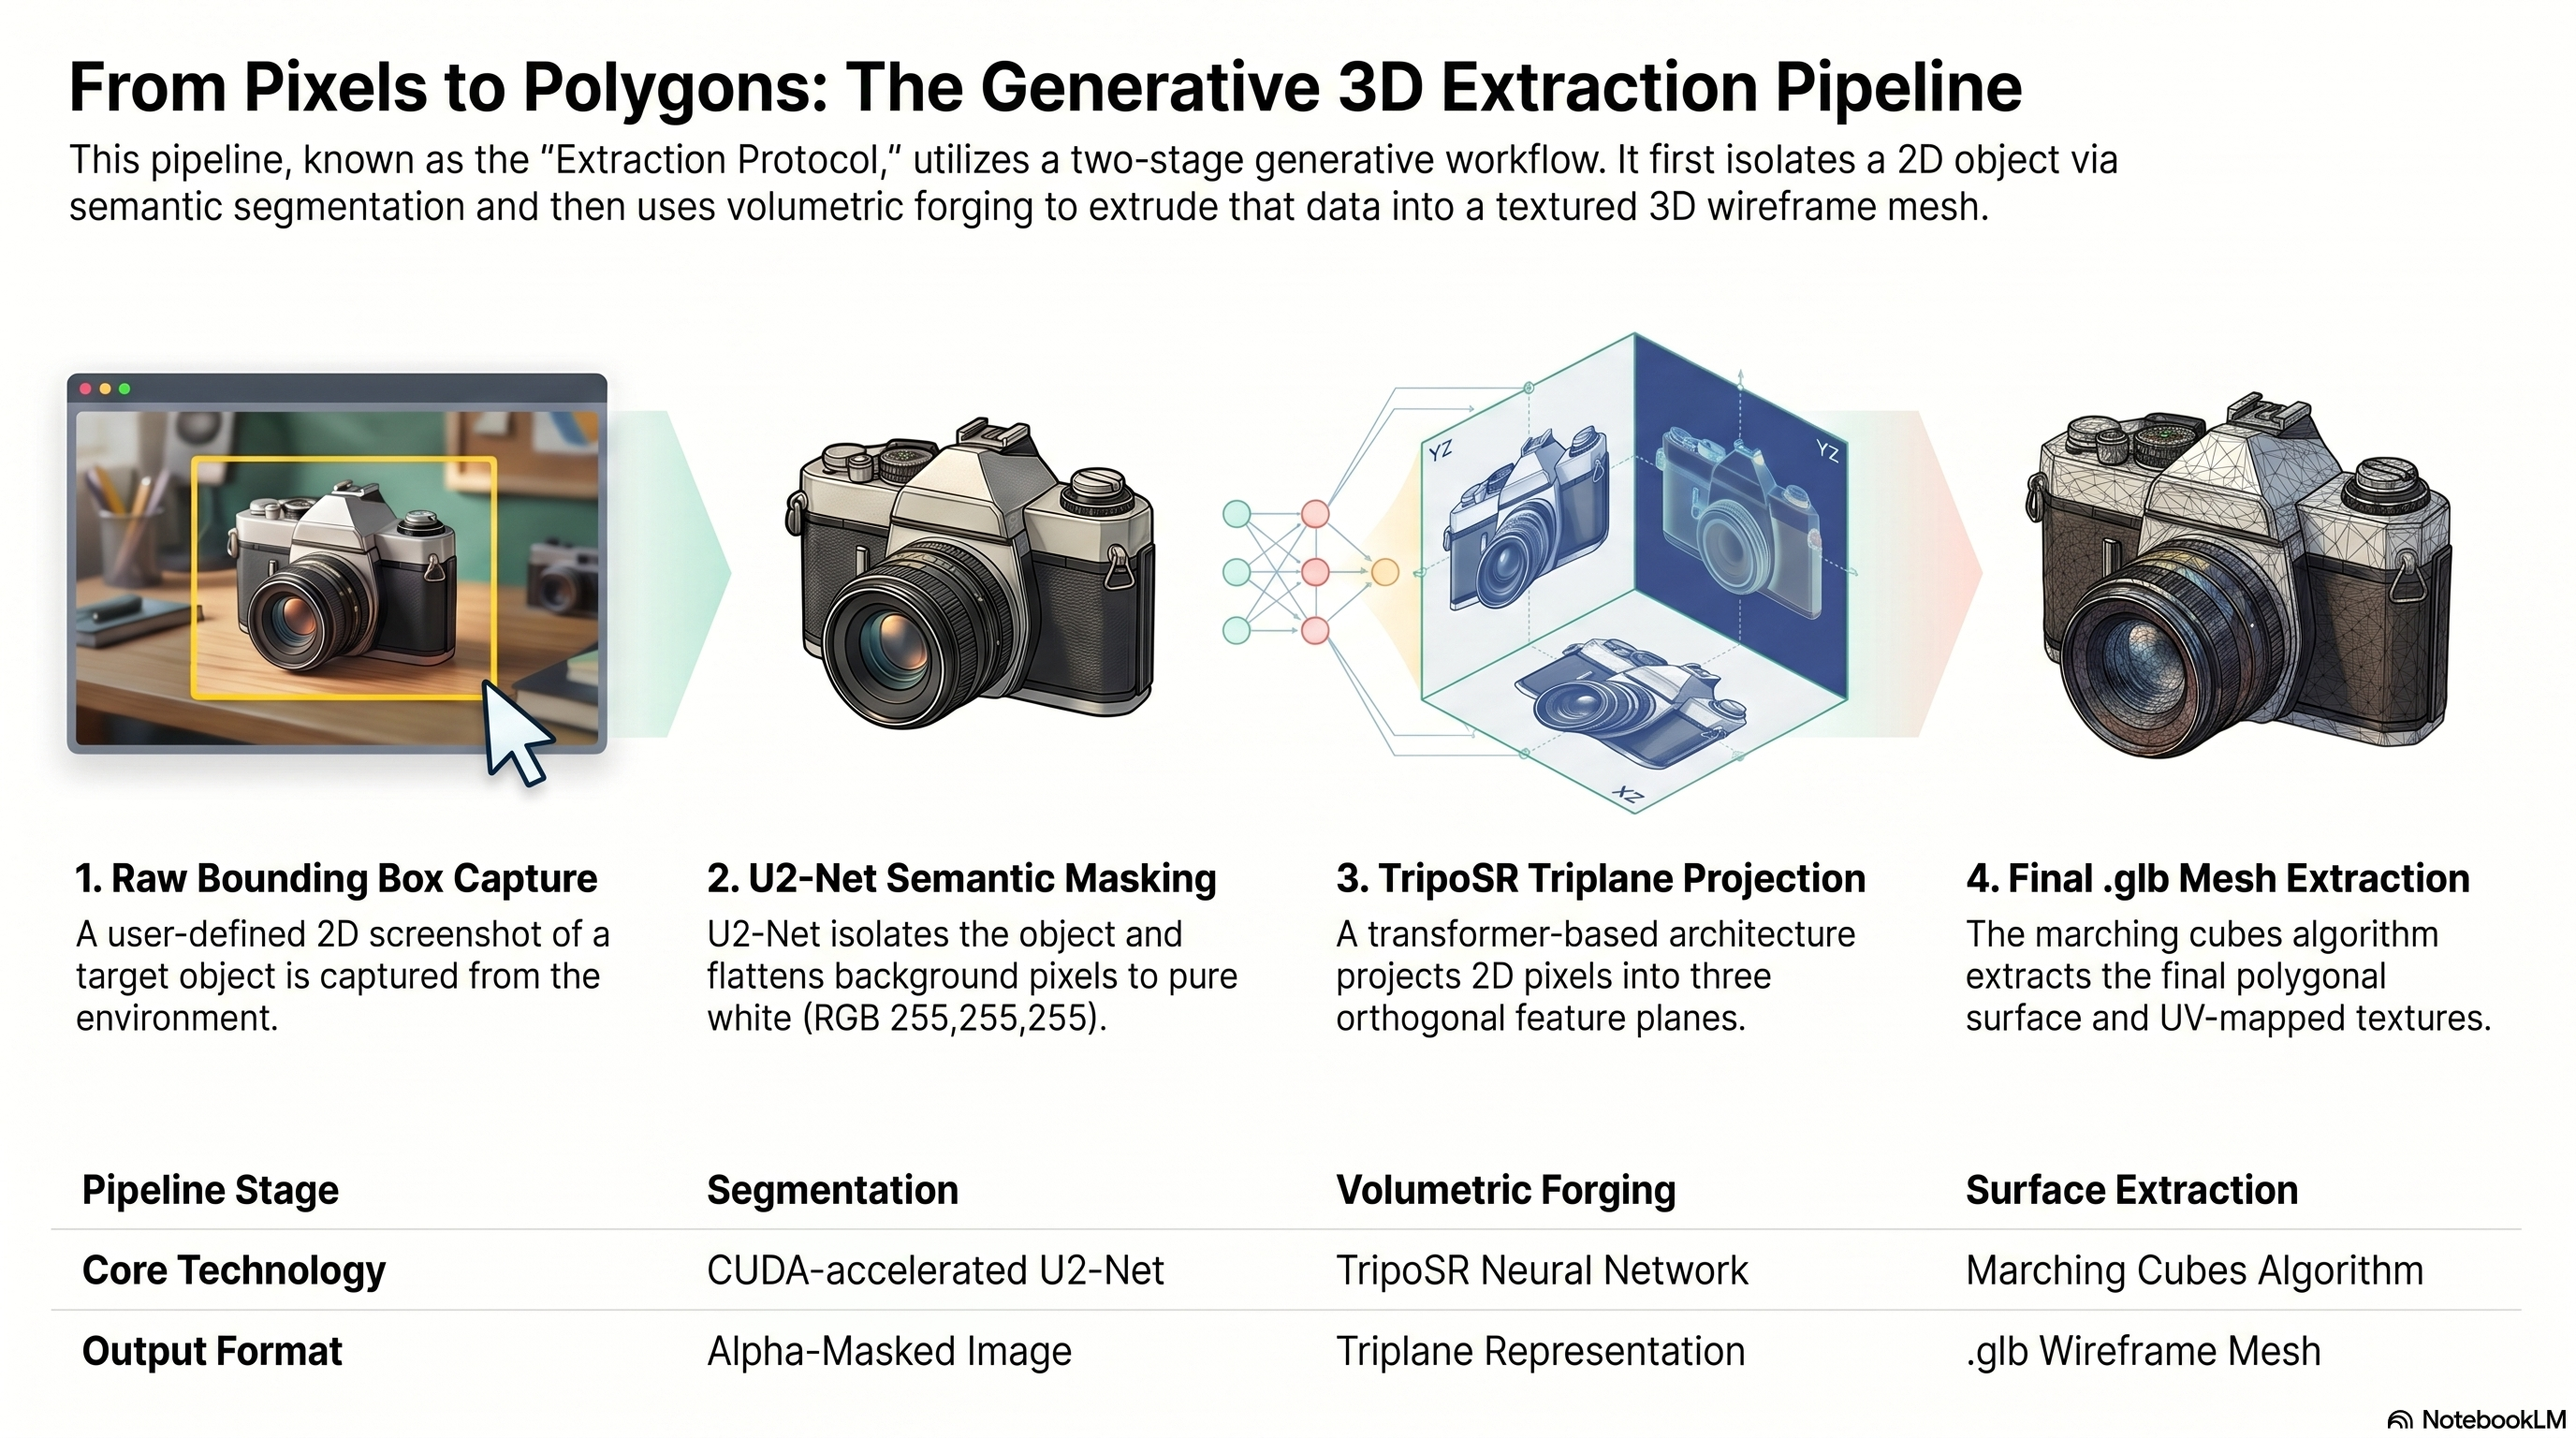
\includegraphics[width=\linewidth]{img/11.png}
    \caption{Created by NotebookLM - The Generative 3D Extraction Pipeline (Scenario 1). This sequential flowchart illustrates the transformation of a raw 2D viewport selection into a fully textured 3D model. The process details the initial semantic segmentation via U\textsuperscript{2}-Net (enforcing a pure white background), followed by volumetric forging and surface extraction utilizing the TripoSR neural network and the marching cubes algorithm.}
    \label{fig:imgto3d}
\end{figure}

% CHANGED TO [H] TO GLUE THE IMAGE EXACTLY HERE
\begin{figure}[H] 
    \centering
    \includegraphics[width=\linewidth]{img/12.png}
    \caption{Created by NotebookLM - The Deep Splat Excavation "hole-punch" process. This overlay demonstrates the mathematical translation of a 2D user selection into a 3D volumetric mask, allowing new assets to be spawned without visual clipping or Z-fighting with the original scanned environment.}
    \label{fig:dbselogo}
\end{figure}

\vspace{0.5cm}
The corresponding JavaScript implementation for this viewport capture protocol is provided in Listing \ref{lst:capture}.

\begin{lstlisting}[language=Java, caption={JavaScript Implementation of captureSelectionSnapshot()}, label={lst:capture}]
function captureSelectionSnapshot(bb) {
    try {
        const prevBg = scene.background ? scene.background.clone() : null;
        const prevFog = scene.fog;
        const prevGridVisible = gridHelper.visible;

        // Isolate canvas for clean extraction
        scene.background = new THREE.Color(0xffffff);
        scene.fog = null;
        gridHelper.visible = false;

        renderer.render(scene, camera);

        const srcCanvas = renderer.domElement;
        const rect = srcCanvas.getBoundingClientRect();
        
        // Map 2D bounds to WebGL coordinates
        const scaleX = srcCanvas.width / rect.width;
        const scaleY = srcCanvas.height / rect.height;
        const clampedW = Math.min(Math.round(bb.w * scaleX), srcCanvas.width);
        const clampedH = Math.min(Math.round(bb.h * scaleY), srcCanvas.height);

        const offCanvas = document.createElement('canvas');
        offCanvas.width = clampedW;
        offCanvas.height = clampedH;
        const offCtx = offCanvas.getContext('2d');
        
        // Extract pixels
        offCtx.drawImage(srcCanvas, Math.round((bb.x - rect.left) * scaleX), Math.round((bb.y - rect.top) * scaleY), clampedW, clampedH, 0, 0, clampedW, clampedH);
        const dataURL = offCanvas.toDataURL('image/png');

        // Restore environment variables
        scene.background = prevBg;
        scene.fog = prevFog;
        gridHelper.visible = prevGridVisible;
        renderer.render(scene, camera);

        // Transmit to FastAPI Backend
        fetch('/api-fastapi/extract', {
            method: 'POST',
            headers: { 'Content-Type': 'application/json' },
            body: JSON.stringify({ image: dataURL })
        }).then(response => response.arrayBuffer())
          .then(arrayBuffer => {
              // Parse and inject generated GLB mesh
              const loader = new GLTFLoader();
              loader.parse(arrayBuffer, '', (gltf) => {
                  scene.add(gltf.scene);
              });
          });
    } catch (err) {
        console.error('[SYSTEM_ERR] Snapshot failed:', err.message);
    }
}
\end{lstlisting}

\newpage
\subsection{A.2 The Summoning Engine: Text-to-3D Orchestration}

Operating heavy generative models strictly within an 8GB VRAM constraint requires the aggressive memory management strategy depicted in Figure \ref{fig:txt23d}. 

% CHANGED TO [H] TO GLUE THE IMAGE EXACTLY HERE
\begin{figure}[H] 
    \centering
    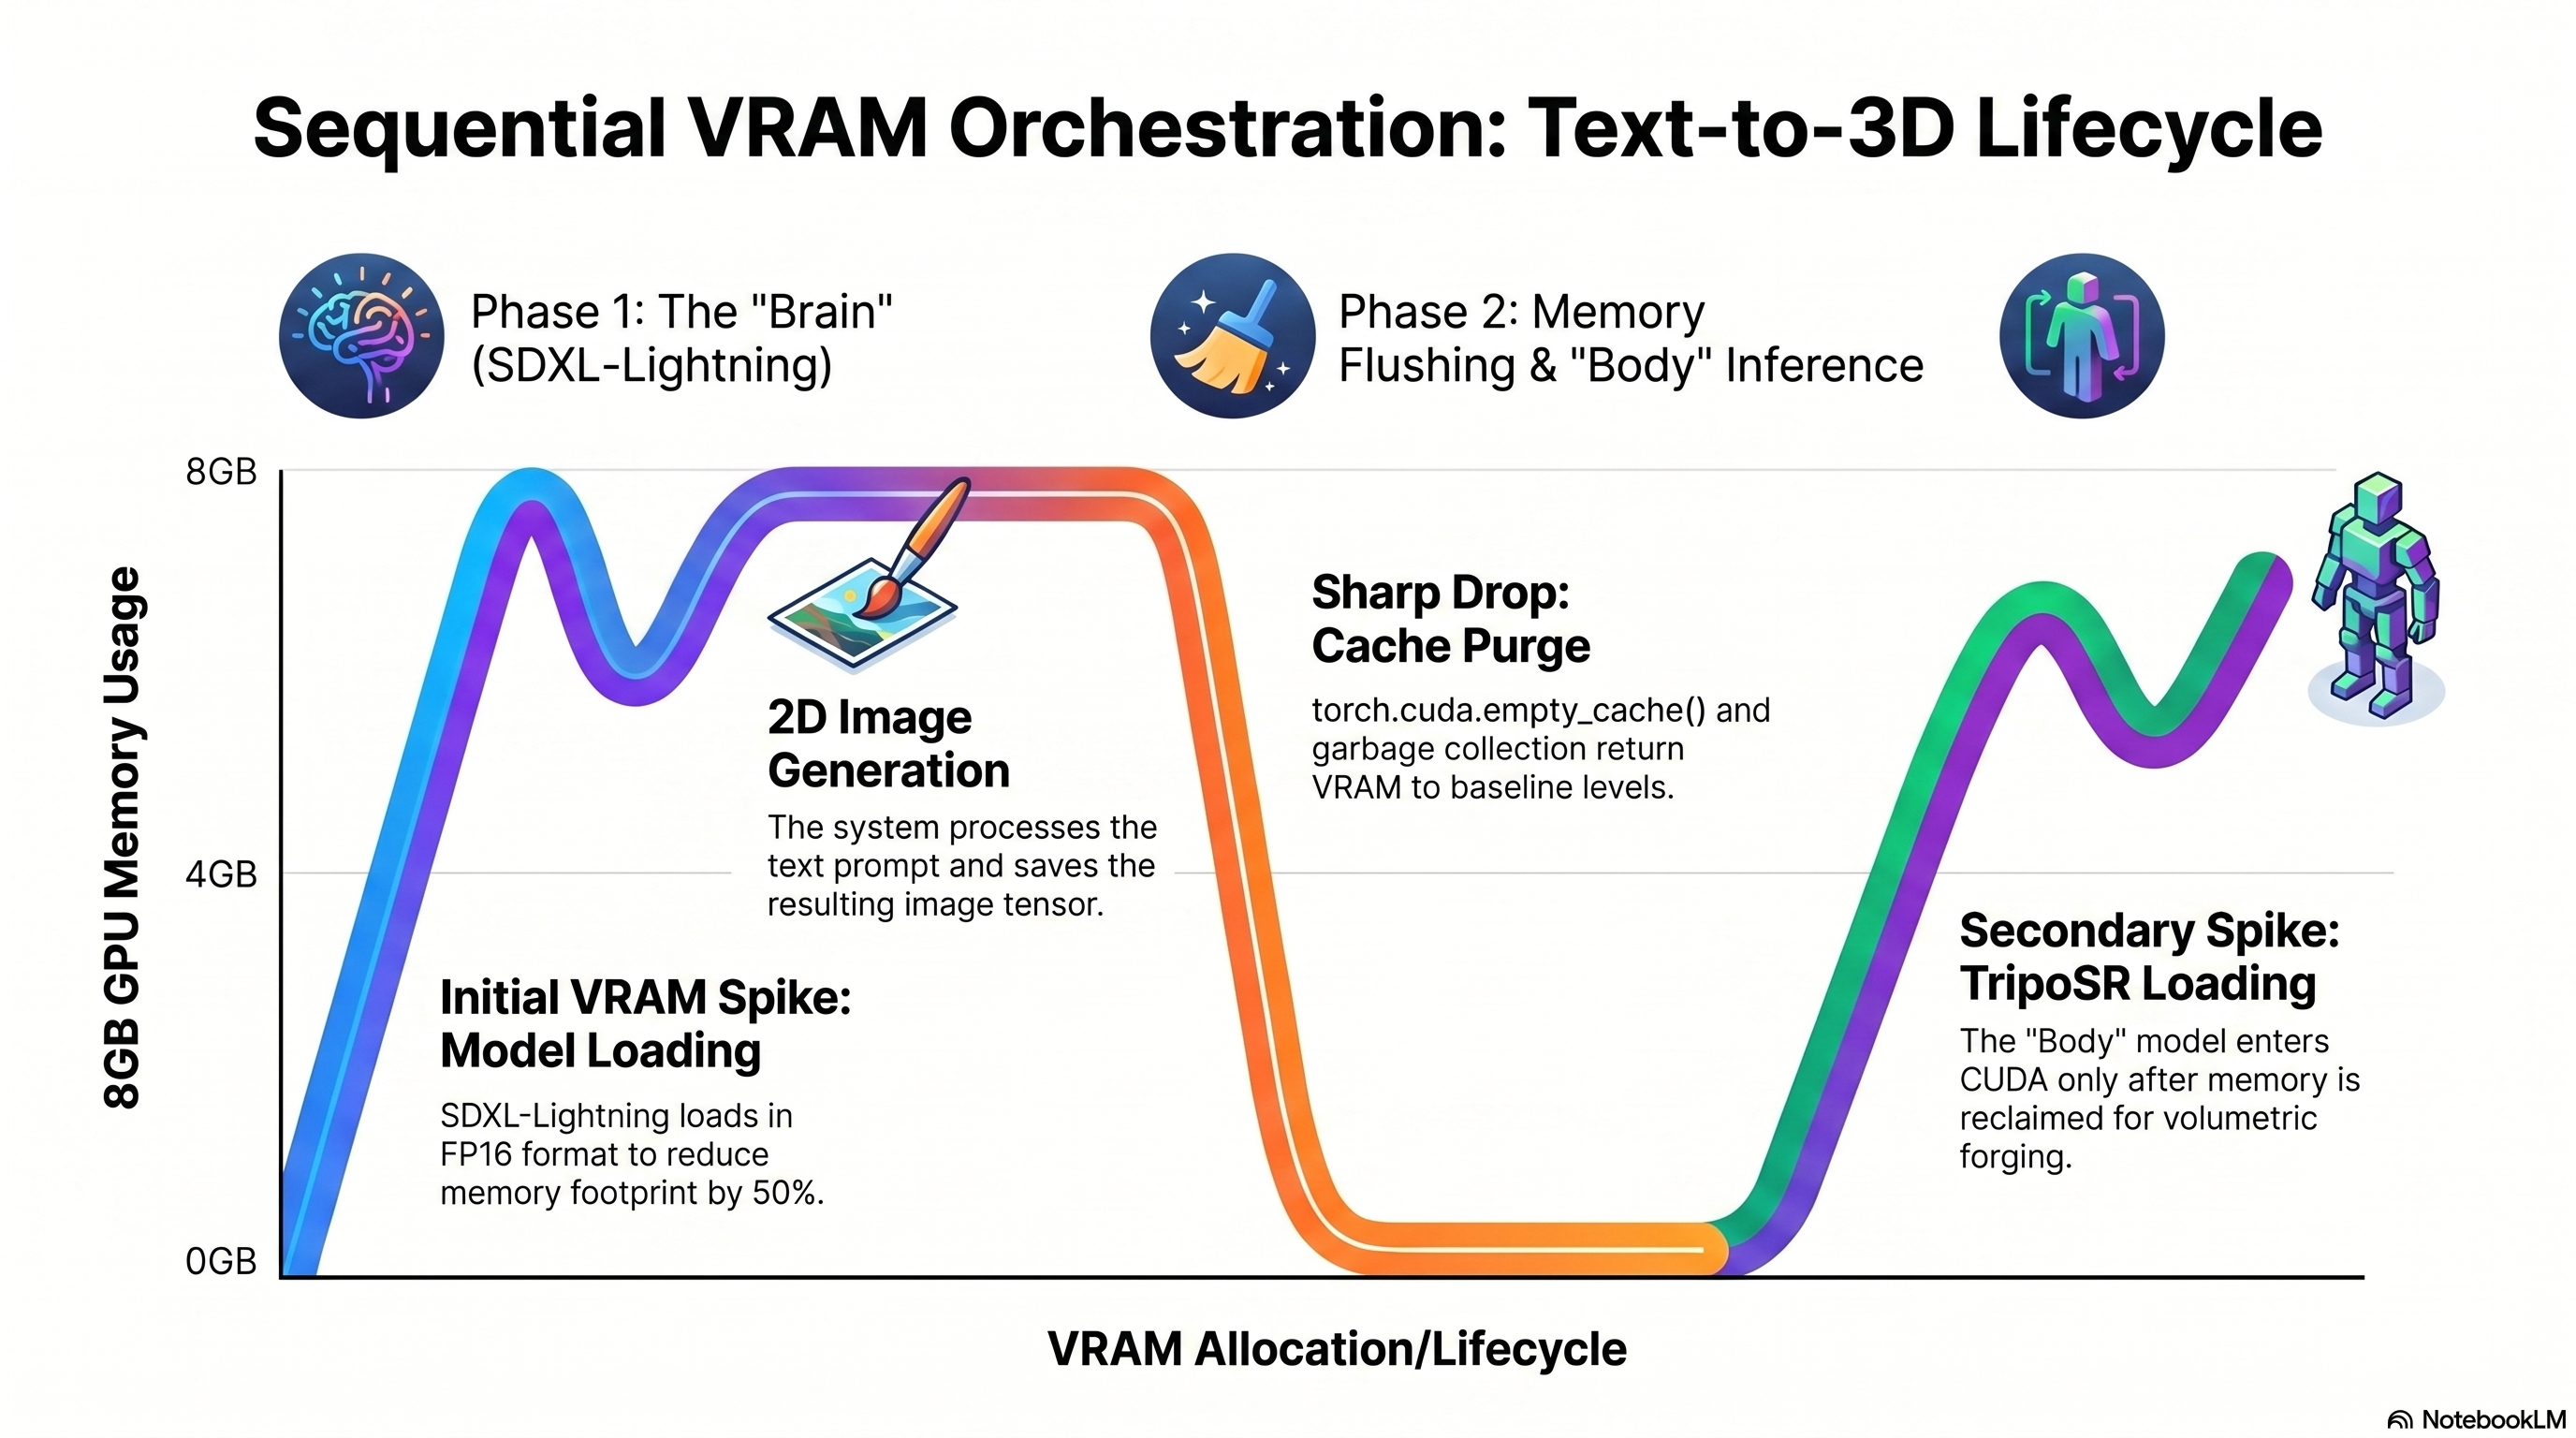
\includegraphics[width=\linewidth]{img/13.png}
    \caption{Created by NotebookLM - Sequential VRAM Orchestration during the Text-to-3D Lifecycle. The graph demonstrates the aggressive memory management strategy required to operate within an 8GB GPU threshold. It highlights the initial VRAM spike during SDXL-Lightning inference, the critical cache purge (\texttt{torch.cuda.empty\_cache()}), and the subsequent memory reallocation for TripoSR volumetric forging.}
    \label{fig:txt23d}
\end{figure}

\vspace{0.5cm}
The asynchronous client-side fetch requests and geometry parsing functions handling this orchestration are detailed in Listing \ref{lst:summon}.

\begin{lstlisting}[language=Java, caption={JavaScript Implementation of executePromptSummon()}, label={lst:summon}]
function executePromptSummon() {
    const prompt = creatorPromptInput.value.trim();
    if (!prompt) return;
    
    showCreatorLoader('Connecting to Stable Diffusion SD3 generator...', 15);
    
    fetch('/api-proxy/summon', {
        method: 'POST',
        headers: { 'Content-Type': 'application/json' },
        body: JSON.stringify({ prompt: prompt })
    })
    .then(response => {
        if (!response.ok) throw new Error(`HTTP ${response.status}`);
        showCreatorLoader('Image generated. Forging 3D geometry locally via TripoSR...', 55);
        return response.arrayBuffer();
    })
    .then(arrayBuffer => {
        showCreatorLoader('Reconstruction complete. Loading 3D spatial mesh...', 85);
        
        const loader = new GLTFLoader();
        loader.parse(arrayBuffer, '', (gltf) => {
            const model = gltf.scene;
            
            // Calculate target spawn point derived from camera forward vector
            const forward = new THREE.Vector3();
            camera.getWorldDirection(forward);
            const targetPos = new THREE.Vector3().copy(camera.position).addScaledVector(forward, 5);
            model.position.copy(targetPos);
            
            // Hide Gaussian Splat environment to reveal standalone mesh
            if (viewer && viewer.splatMesh) viewer.splatMesh.visible = false;
            
            scene.add(model);
            hideCreatorLoader();
        });
    })
    .catch(err => {
        console.error('SYS_ERR: Summon failed:', err.message);
        hideCreatorLoader();
    });
}
\end{lstlisting}

\end{document}
